

The theory behind implementation and design of Solomonoff has been studied and developed over the course of 2 years. The early versions and our initial ideas looked very different to the final results we've achieved. 

At the beginning it was meant to be a simple tool that focused only on deterministic Mealy automata. Such a model was very limited and it quickly became apparent that certain extensions would be necessary. In the end we implemented a compiler that supports nondeterministic functional weighted symbolic transducers. 

\section{Mealy automata and transducers}

The standard definition of automaton found in introductory courses \cite{sipser, EILENBERG,EILENBERG2} states that finite state automaton is  a tuple $(Q,I,\delta,F,\Sigma)$ where $Q$ is the set of states, $I \subset Q$ are the initial states,  $F \subset Q$ are the final (or accepting) states, $\delta:Q\times \Sigma \rightarrow Q$ is the transition function and $\Sigma$ is some alphabet. The automaton can either accept or reject a certain input string. Below is an example in the form of a state graph.

\begin{center}
	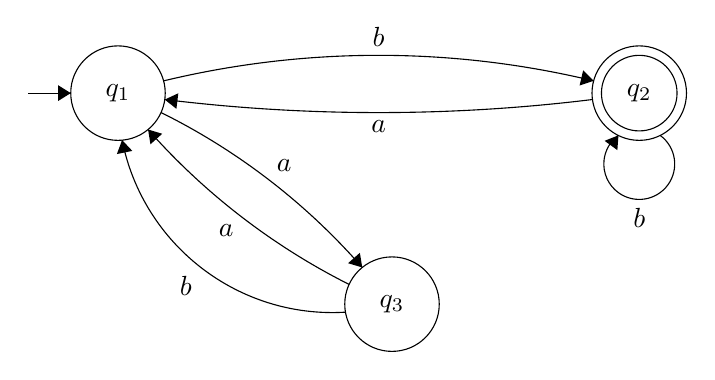
\begin{tikzpicture}[scale=0.2]
		\tikzstyle{every node}+=[inner sep=0pt]
		\draw [black] (18.8,-23.1) circle (3);
		\draw (18.8,-23.1) node {$q_1$};
		\draw [black] (51.9,-23.1) circle (3);
		\draw (51.9,-23.1) node {$q_2$};
		\draw [black] (51.9,-23.1) circle (2.4);
		\draw [black] (36.2,-36.5) circle (3);
		\draw (36.2,-36.5) node {$q_3$};
		\draw [black] (21.697,-22.322) arc (103.55817:76.44183:58.239);
		\fill [black] (49,-22.32) -- (48.34,-21.65) -- (48.11,-22.62);
		\draw (35.35,-20.2) node [above] {$b$};
		\draw [black] (21.534,-24.333) arc (63.64958:41.14961:41.326);
		\fill [black] (34.31,-34.17) -- (34.16,-33.24) -- (33.41,-33.9);
		\draw (29.36,-28.13) node [above] {$a$};
		\draw [black] (33.475,-35.247) arc (-116.70226:-138.49855:42.617);
		\fill [black] (20.71,-25.41) -- (20.86,-26.35) -- (21.61,-25.68);
		\draw (25.67,-31.44) node [below] {$a$};
		\draw [black] (48.928,-23.506) arc (-82.99966:-97.00034:111.406);
		\fill [black] (21.77,-23.51) -- (22.51,-24.1) -- (22.63,-23.11);
		\draw (35.35,-24.84) node [below] {$a$};
		\draw [black] (33.25,-37.01) arc (-86.50408:-168.69673:13.623);
		\fill [black] (19.06,-26.08) -- (18.73,-26.97) -- (19.71,-26.77);
		\draw (23.1,-34.7) node [below] {$b$};
		\draw [black] (53.223,-25.78) arc (54:-234:2.25);
		\draw (51.9,-30.35) node [below] {$b$};
		\fill [black] (50.58,-25.78) -- (49.7,-26.13) -- (50.51,-26.72);
		\draw [black] (13.1,-23.1) -- (15.8,-23.1);
		\fill [black] (15.8,-23.1) -- (15,-22.6) -- (15,-23.6);
	\end{tikzpicture}
\end{center}
The accepting state $q_2\in F$ is marked with a double border. Such automaton accepts strings like $bb$,$bbb$,$bab$,$aab$ but rejects $\epsilon$,$a$,$ba$,$aa$ and so on. 

A Mealy machine \cite{mealy} extends the above definition with output  $(Q,I,\delta,F,\Sigma,\Gamma)$ where $\Gamma$ is some output alphabet and transition function has the form of $\delta:Q\times \Sigma \rightarrow Q \times \Gamma$. For example the below machine
\begin{center}
	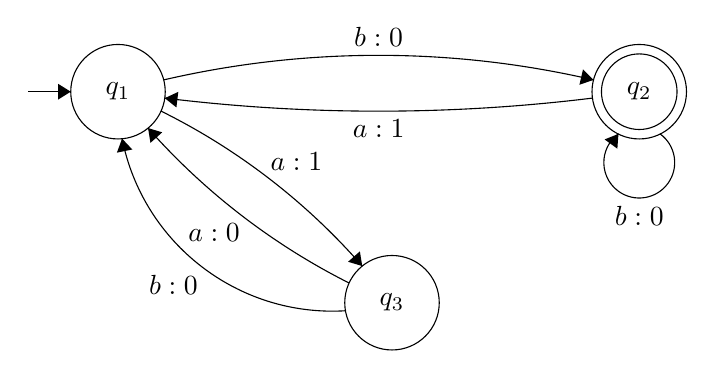
\begin{tikzpicture}[scale=0.2]
		\tikzstyle{every node}+=[inner sep=0pt]
		\draw [black] (18.8,-23.1) circle (3);
		\draw (18.8,-23.1) node {$q_1$};
		\draw [black] (51.9,-23.1) circle (3);
		\draw (51.9,-23.1) node {$q_2$};
		\draw [black] (51.9,-23.1) circle (2.4);
		\draw [black] (36.2,-36.5) circle (3);
		\draw (36.2,-36.5) node {$q_3$};
		\draw [black] (21.704,-22.35) arc (103.05311:76.94689:60.417);
		\fill [black] (49,-22.35) -- (48.33,-21.68) -- (48.1,-22.66);
		\draw (35.35,-20.29) node [above] {$b:0$};
		\draw [black] (21.534,-24.333) arc (63.64958:41.14961:41.326);
		\fill [black] (34.31,-34.17) -- (34.16,-33.24) -- (33.41,-33.9);
		\draw (30.13,-28.13) node [above] {$a:1$};
		\draw [black] (33.475,-35.247) arc (-116.70226:-138.49855:42.617);
		\fill [black] (20.71,-25.41) -- (20.86,-26.35) -- (21.61,-25.68);
		\draw (24.9,-31.44) node [below] {$a:0$};
		\draw [black] (48.928,-23.506) arc (-82.99966:-97.00034:111.406);
		\fill [black] (21.77,-23.51) -- (22.51,-24.1) -- (22.63,-23.11);
		\draw (35.35,-24.84) node [below] {$a:1$};
		\draw [black] (33.25,-37.01) arc (-86.50408:-168.69673:13.623);
		\fill [black] (19.06,-26.08) -- (18.73,-26.97) -- (19.71,-26.77);
		\draw (22.32,-34.7) node [below] {$b:0$};
		\draw [black] (53.223,-25.78) arc (54:-234:2.25);
		\draw (51.9,-30.35) node [below] {$b:0$};
		\fill [black] (50.58,-25.78) -- (49.7,-26.13) -- (50.51,-26.72);
		\draw [black] (13.1,-23.1) -- (15.8,-23.1);
		\fill [black] (15.8,-23.1) -- (15,-22.6) -- (15,-23.6);
	\end{tikzpicture}
\end{center}
produces output $1000$ for input $aabb$. Some articles do not include the set $F$ in definition of Mealy machines and instead assume that all states are accepting. Automata with all states final are called prefix-closed. Here we do not assume Mealy machines to be prefix-closed.

The ability to produce output along each transition allows for modelling reactive systems. Any program or phenomenon that reads input from it's environment and ``reacts'' to it by producing output in one form or another is a reactive system. It is frequently used in the field of formal methods. Many complex state-based systems can be modelled and simplified using Mealy machines \cite{de_la_higuera}. As an example consider a black-box computer program whose logs can be observed \cite{register_automata_learning}. The current snapshot of the program's memory determines its state. Depending on subsequent user input, we might observe different log traces. There are many existing machine learning and inference algorithms that can build an equivalent model of Mealy machine only by interacting with such a black-box system and reading its logs. 

It can be proved that the expressive power of deterministic automata with output is strictly less than that of their nondeterministic counterparts \cite{MendozaDrosik2020MultitapeAA}. It is known as the prefix-preserving  property \cite{de_la_higuera}. If a deterministic automaton reads input string $\sigma_1\sigma_2\sigma_1$ and prints $\gamma_1\gamma_1\gamma_2$, then at the next step it is only allowed to append one more symbol to the previously generated output. For instance we could not suddenly change the output to $\gamma_2\gamma_2\gamma_2\gamma_1$ after reading one more input symbol $\sigma_1\sigma_2\sigma_1\sigma_2$. The prefix $\gamma_1\gamma_1\gamma_2$ must be preserved. 

The problems that we wanted to tackle with Solomonoff revolved around building sequence-to-sequence models. For instance we might want to translate from numbers written as English words into digits. A sentence like ``zero bugs'' should become ``0 bugs''. The prefix preserving property would be too limiting because it often happens that the suffix of string has a decisive impact on the translation. The phrase ``zeroed bit''
also starts with the prefix ``zero'' but it should not be translated as ``0ed bit''!

We intended to find the right balance between expressive power of nondeterministic machines and strong formal guarantees of Mealy automata. To achieve this, we initially decided to use multitape automata \cite{TRANSDUCERS}. 
For example the automaton below has 4 tapes
\begin{center}
	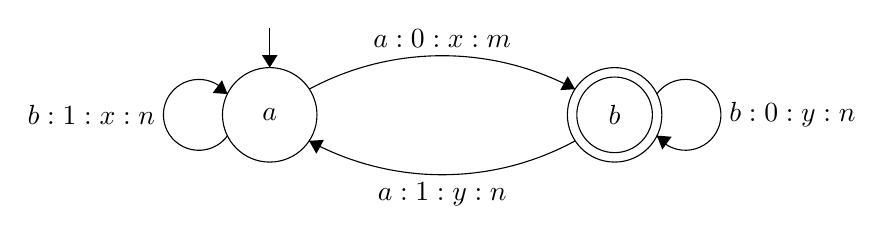
\begin{tikzpicture}[scale=0.2]
		\tikzstyle{every node}+=[inner sep=0pt]
		\draw [black] (29.2,-14.2) circle (3);
		\draw (29.2,-14.2) node {$a$};
		\draw [black] (51.1,-14.2) circle (3);
		\draw (51.1,-14.2) node {$b$};
		\draw [black] (51.1,-14.2) circle (2.4);
		\draw [black] (31.712,-12.566) arc (118.22602:61.77398:17.842);
		\fill [black] (48.59,-12.57) -- (48.12,-11.75) -- (47.65,-12.63);
		\draw (40.15,-9.94) node [above] {$a:0:x:m$};
		\draw [black] (48.6,-15.851) arc (-61.42174:-118.57826:17.664);
		\fill [black] (31.7,-15.85) -- (32.16,-16.67) -- (32.64,-15.79);
		\draw (40.15,-18.5) node [below] {$a:1:y:n$};
		\draw [black] (53.78,-12.877) arc (144:-144:2.25);
		\draw (58.35,-14.2) node [right] {$b:0:y:n$};
		\fill [black] (53.78,-15.52) -- (54.13,-16.4) -- (54.72,-15.59);
		\draw [black] (26.52,-15.523) arc (324:36:2.25);
		\draw (21.95,-14.2) node [left] {$b:1:x:n$};
		\fill [black] (26.52,-12.88) -- (26.17,-12) -- (25.58,-12.81);
		\draw [black] (29.2,-8.7) -- (29.2,-11.2);
		\fill [black] (29.2,-11.2) -- (29.7,-10.4) -- (28.7,-10.4);
	\end{tikzpicture}
\end{center}
First tape is designated as the input state reading strings over the alphabet $\{a,b\}$. The remaining three tapes are the output tapes, printing strings in the respective alphabets $\{0,1\}$, $\{x,y\}$, $\{m,n\}$. In theory there could be any (finite) number of input and output tapes. 

Our idea was to write all possible continuations of given output and store each in a separate output tape. Then upon reaching the end of string, the state would decide which tape to use as output. 

Over the course of research and development we have discovered that the power of multitape Mealy machines was still too limiting for our purposes. In particular we could define congruence classes on pairs of strings similar to those in Myhill-Nerode theorem \cite{sipser}. Then it can be easily noticed that as long as the number of output tapes is finite, the number of congruence classes must be finite as well. A very simple and intuitive counter-example would be the language that for every string $a$, $aa$, $aaa$,... respectively prints output $c$, $bc$, $bbc$,... and so on. It could not be expressed using any finite number of output tapes, because there are infinitely many ways to continue the output and none of them is a prefix of the other.  



Yet another limitation of Mealy machines is that their $\delta$ function enforces outputs of the exact same length as inputs. In the field of natural language processing such an assumption is too strict. For instance, we might want to 
build a machine that translates sentences from one language to another. A word ``fish'' in English might have 4 letters but Spanish ``pescado'' is much longer. Our first idea was to use sequential transducers instead of the plain Mealy automata. Their definition allows the transition function to print output strings of arbitrary length $\delta:Q\times \Sigma \rightarrow Q^*$.  


The nondeterministic transducers \cite{MOHRI} \cite{MOHRI2} \cite{MOHRI3}  don't suffer from any of the above problems. Their expressive power exactly corresponds to that of regular transductions. It's a very strong and expressive class. The only way to obtain a stronger model would be by introducing context-free grammars and pushdown automata. The reason why we were hesitant to use this approach was because of the possible ambiguity of output \cite{Marie-Pierre}. Nondeterministic transducers may contain epsilon transitions, which could lead to infinite number of outputs \cite{MendozaDrosik2020MultitapeAA} for any given input. Without epsilons, the number of outputs is finite but it's still possible to return more than one ambiguous output. 


The hierarchy of automata presented so far could be illustrated as follows.
\begin{center}
\end{center}



\tikzset{every picture/.style={line width=0.75pt}} %set default line width to 0.75pt        

\begin{tikzpicture}[x=0.75pt,y=0.75pt,yscale=-1,xscale=1]
	%uncomment if require: \path (0,235); %set diagram left start at 0, and has height of 235
	
	
	% Text Node
	\draw (129,40) node    {$Mealy\ Machines$};
	% Text Node
	\draw (53,111) node    {$ \begin{array}{l}
			Sequential\ \\
			transducers
		\end{array}$};
	% Text Node
	\draw (211,110) node    {$ \begin{array}{l}
			Multitape\\
			Mealy\ Machines
		\end{array}$};
	% Text Node
	\draw (127,181) node    {$ \begin{array}{l}
			Nondeterministic\\
			transducers
		\end{array}$};
	% Text Node
	\draw (721,21) node    {$0$};
	% Text Node
	\draw (701,71) node    {$0$};
	% Connection
	\draw    (143.06,52) -- (183.71,86.7) ;
	\draw [shift={(185.23,88)}, rotate = 220.49] [color={rgb, 255:red, 0; green, 0; blue, 0 }  ][line width=0.75]    (10.93,-3.29) .. controls (6.95,-1.4) and (3.31,-0.3) .. (0,0) .. controls (3.31,0.3) and (6.95,1.4) .. (10.93,3.29)   ;
	% Connection
	\draw    (116.15,52) -- (78.01,87.63) ;
	\draw [shift={(76.55,89)}, rotate = 316.95] [color={rgb, 255:red, 0; green, 0; blue, 0 }  ][line width=0.75]    (10.93,-3.29) .. controls (6.95,-1.4) and (3.31,-0.3) .. (0,0) .. controls (3.31,0.3) and (6.95,1.4) .. (10.93,3.29)   ;
	% Connection
	\draw    (76.26,133) -- (102.29,157.63) ;
	\draw [shift={(103.74,159)}, rotate = 223.41] [color={rgb, 255:red, 0; green, 0; blue, 0 }  ][line width=0.75]    (10.93,-3.29) .. controls (6.95,-1.4) and (3.31,-0.3) .. (0,0) .. controls (3.31,0.3) and (6.95,1.4) .. (10.93,3.29)   ;
	% Connection
	\draw    (184.97,132) -- (154.56,157.71) ;
	\draw [shift={(153.03,159)}, rotate = 319.78999999999996] [color={rgb, 255:red, 0; green, 0; blue, 0 }  ][line width=0.75]    (10.93,-3.29) .. controls (6.95,-1.4) and (3.31,-0.3) .. (0,0) .. controls (3.31,0.3) and (6.95,1.4) .. (10.93,3.29)   ;
	
\end{tikzpicture}
\begin{center}
	
\end{center}
Mealy machines are the simplest and most basic model. Both sequential transducers and multitape automata extend the expressive power of Mealy machines in different ways but neither is more powerful than the other. Finally, nondeterministic transducers are on top of the hierarchy. This is a simplified view. The full family of different models capable of producing output is much larger. The transduction hierarchy is more complex than Chomsky hierarchy, even within the layer of regular transductions (not to mention context-free and context-sensitive transductions).   

The model of automata that was finally implemented in Solomonoff, is the functional nondeterministic transducer \cite{TRANSDUCERS}. Functionality of a transducer means that for any input, there may be at most one output. For instance the transducer below is not functional, because for input string $abb$ it prints both outputs $xyx$ and $yxx$. 
\begin{center}
	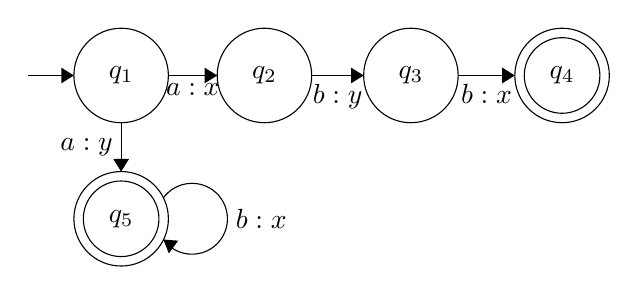
\begin{tikzpicture}[scale=0.2]
		\tikzstyle{every node}+=[inner sep=0pt]
		\draw [black] (40.2,-18) circle (3);
		\draw (40.2,-18) node {$q_4$};
		\draw [black] (40.2,-18) circle (2.4);
		\draw [black] (12.2,-18) circle (3);
		\draw (12.2,-18) node {$q_1$};
		\draw [black] (21.3,-18) circle (3);
		\draw (21.3,-18) node {$q_2$};
		\draw [black] (12.2,-27.1) circle (3);
		\draw (12.2,-27.1) node {$q_5$};
		\draw [black] (12.2,-27.1) circle (2.4);
		\draw [black] (30.6,-18) circle (3);
		\draw (30.6,-18) node {$q_3$};
		\draw [black] (15.2,-18) -- (18.3,-18);
		\fill [black] (18.3,-18) -- (17.5,-17.5) -- (17.5,-18.5);
		\draw (16.75,-18.5) node [below] {$a:x$};
		\draw [black] (6.3,-18) -- (9.2,-18);
		\fill [black] (9.2,-18) -- (8.4,-17.5) -- (8.4,-18.5);
		\draw [black] (24.3,-18) -- (27.6,-18);
		\fill [black] (27.6,-18) -- (26.8,-17.5) -- (26.8,-18.5);
		\draw (25.95,-18.5) node [below] {$b:y$};
		\draw [black] (33.6,-18) -- (37.2,-18);
		\fill [black] (37.2,-18) -- (36.4,-17.5) -- (36.4,-18.5);
		\draw (35.4,-18.5) node [below] {$b:x$};
		\draw [black] (12.2,-21) -- (12.2,-24.1);
		\fill [black] (12.2,-24.1) -- (12.7,-23.3) -- (11.7,-23.3);
		\draw (11.7,-22.55) node [left] {$a:y$};
		\draw [black] (14.88,-25.777) arc (144:-144:2.25);
		\draw (19.45,-27.1) node [right] {$b:x$};
		\fill [black] (14.88,-28.42) -- (15.23,-29.3) -- (15.82,-28.49);
	\end{tikzpicture}
\end{center}
This should not be confused with unambiguous automata. For example the transducer below is functional but ambiguous. The input $abb$ prints only a single output $yxx$, albeit there are two ambiguous accepting paths that produce it.
\begin{center}
	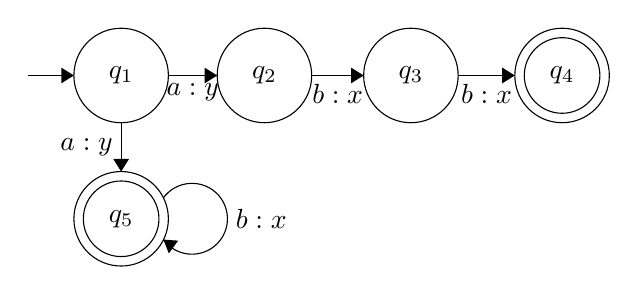
\begin{tikzpicture}[scale=0.2]
		\tikzstyle{every node}+=[inner sep=0pt]
		\draw [black] (40.2,-18) circle (3);
		\draw (40.2,-18) node {$q_4$};
		\draw [black] (40.2,-18) circle (2.4);
		\draw [black] (12.2,-18) circle (3);
		\draw (12.2,-18) node {$q_1$};
		\draw [black] (21.3,-18) circle (3);
		\draw (21.3,-18) node {$q_2$};
		\draw [black] (12.2,-27.1) circle (3);
		\draw (12.2,-27.1) node {$q_5$};
		\draw [black] (12.2,-27.1) circle (2.4);
		\draw [black] (30.6,-18) circle (3);
		\draw (30.6,-18) node {$q_3$};
		\draw [black] (15.2,-18) -- (18.3,-18);
		\fill [black] (18.3,-18) -- (17.5,-17.5) -- (17.5,-18.5);
		\draw (16.75,-18.5) node [below] {$a:y$};
		\draw [black] (6.3,-18) -- (9.2,-18);
		\fill [black] (9.2,-18) -- (8.4,-17.5) -- (8.4,-18.5);
		\draw [black] (24.3,-18) -- (27.6,-18);
		\fill [black] (27.6,-18) -- (26.8,-17.5) -- (26.8,-18.5);
		\draw (25.95,-18.5) node [below] {$b:x$};
		\draw [black] (33.6,-18) -- (37.2,-18);
		\fill [black] (37.2,-18) -- (36.4,-17.5) -- (36.4,-18.5);
		\draw (35.4,-18.5) node [below] {$b:x$};
		\draw [black] (12.2,-21) -- (12.2,-24.1);
		\fill [black] (12.2,-24.1) -- (12.7,-23.3) -- (11.7,-23.3);
		\draw (11.7,-22.55) node [left] {$a:y$};
		\draw [black] (14.88,-25.777) arc (144:-144:2.25);
		\draw (19.45,-27.1) node [right] {$b:x$};
		\fill [black] (14.88,-28.42) -- (15.23,-29.3) -- (15.82,-28.49);
	\end{tikzpicture}
\end{center}
Functional nondeterministic transducers proved to provide the perfect balance of power with many strong formal guarantees. While epsilon transitions strictly increase power of transducers, when restricted only to functional automata, the erasure of epsilons becomes possible (with the exception of epsilon transitions coming from initial state). Using advance-and-delay \cite{Marie-Pierre} algorithm one can test functionality of any automaton in quadratic time. There exists a special version of powerset construction that can take any functional transducers and produce an equivalent unambiguous automaton. One can take advantage of unambiguity to build an inference algorithm for learning functional automata from sample data.  The automata are closed under union, concatenation, Kleene closure and composition. Unlike non-functional transducers, they are not closed under inversion but we developed a special algebra that uniquely defines an invertible  bijective transduction for any automaton. Glushkov's construction \cite{GLUSHKOV} can be augmented to produce functional transducers.  Lexicographic semiring of weights can be used to make functional automata more compact.  


Once we decided to use the power of functional transducers, the next problem we had to solve was their optimisation. One of the most important operations in natural language processing is the context-dependent rewrite. The standard way of implementing it is by building a large transducer that handles all possible cases.
In Solomonoff we've developed our own approach that produces much smaller automata. It is done with lexicographic weights \cite{MendozaDrosik2020MultitapeAA}.

Another important optimisation is the state minimisation. Many existing libraries implement separate functions for all regular operations and additional one for minimisation. A regular expression like $A(B+C)*$ would be then translated to a series of function calls like 
\[
\texttt{minimise}(\texttt{concatenate}(A,\texttt{kleene\_closure}(\texttt{union}(B,C)))) 
\]
This was our initial idea too but later we stumbled upon a better approach. In Solomonoff we don't have separate implementations for those operations. Instead everything is integrated in the form of one monolithic procedure that implements Glushkov's construction. For example, in order to compile the expression
\[
aa(b+ca)*+c
\] we first convert every symbol into a state and obtain the following intermediate ``regular expression'' 
\[
q_1q_2(q_3+q_4 q_5)*+q_6
\]
Then we add one more state at the beginning that will serve as initial
\[
q_0(q_1q_2(q_3+q_4 q_5)*+q_6)
\]
Next we analyse it and determine, which state can be reached from any other. After ``reading'' $q_1$ we can ``read'' $q_2$. After $q_2$ we can either read $q_3$ or $q_4$. After $q_3$ we can read either $q_3$ again or go to $q_4$. Analogically for the remaining states. We also check, which states can appear at the end of the regular expression. In this example $q_2$, $q_3$, $q_5$ and $q_6$ are the final states because reading may end after reaching them. By putting all the above information together, we are able to produce the following automaton.

\begin{center}
	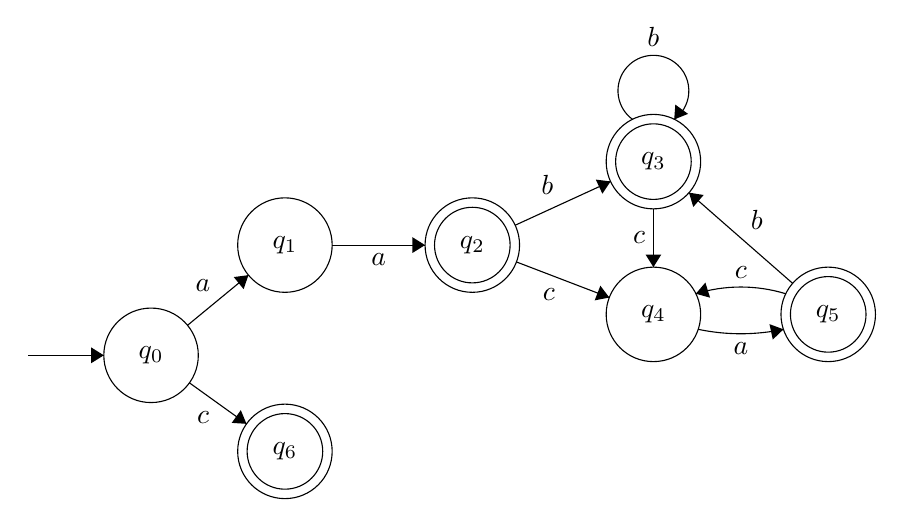
\begin{tikzpicture}[scale=0.2]
		\tikzstyle{every node}+=[inner sep=0pt]
		\draw [black] (21.6,-19.8) circle (3);
		\draw (21.6,-19.8) node {$q_1$};
		\draw [black] (13.1,-26.8) circle (3);
		\draw (13.1,-26.8) node {$q_0$};
		\draw [black] (33.5,-19.8) circle (3);
		\draw (33.5,-19.8) node {$q_2$};
		\draw [black] (33.5,-19.8) circle (2.4);
		\draw [black] (45,-14.5) circle (3);
		\draw (45,-14.5) node {$q_3$};
		\draw [black] (45,-14.5) circle (2.4);
		\draw [black] (45,-24.2) circle (3);
		\draw (45,-24.2) node {$q_4$};
		\draw [black] (56.1,-24.2) circle (3);
		\draw (56.1,-24.2) node {$q_5$};
		\draw [black] (56.1,-24.2) circle (2.4);
		\draw [black] (21.6,-32.9) circle (3);
		\draw (21.6,-32.9) node {$q_6$};
		\draw [black] (21.6,-32.9) circle (2.4);
		\draw [black] (5.3,-26.8) -- (10.1,-26.8);
		\fill [black] (10.1,-26.8) -- (9.3,-26.3) -- (9.3,-27.3);
		\draw [black] (15.42,-24.89) -- (19.28,-21.71);
		\fill [black] (19.28,-21.71) -- (18.35,-21.83) -- (18.98,-22.6);
		\draw (16.4,-22.81) node [above] {$a$};
		\draw [black] (24.6,-19.8) -- (30.5,-19.8);
		\fill [black] (30.5,-19.8) -- (29.7,-19.3) -- (29.7,-20.3);
		\draw (27.55,-20.3) node [below] {$a$};
		\draw [black] (36.22,-18.54) -- (42.28,-15.76);
		\fill [black] (42.28,-15.76) -- (41.34,-15.64) -- (41.76,-16.54);
		\draw (38.27,-16.64) node [above] {$b$};
		\draw [black] (36.3,-20.87) -- (42.2,-23.13);
		\fill [black] (42.2,-23.13) -- (41.63,-22.38) -- (41.27,-23.31);
		\draw (38.36,-22.52) node [below] {$c$};
		\draw [black] (53.261,-25.148) arc (-78.08261:-101.91739:13.126);
		\fill [black] (53.26,-25.15) -- (52.37,-24.82) -- (52.58,-25.8);
		\draw (50.55,-25.93) node [below] {$a$};
		\draw [black] (47.687,-22.893) arc (107.10284:72.89716:9.734);
		\fill [black] (47.69,-22.89) -- (48.6,-23.14) -- (48.3,-22.18);
		\draw (50.55,-21.96) node [above] {$c$};
		\draw [black] (53.84,-22.23) -- (47.26,-16.47);
		\fill [black] (47.26,-16.47) -- (47.53,-17.38) -- (48.19,-16.62);
		\draw (51.56,-18.86) node [above] {$b$};
		\draw [black] (45,-17.5) -- (45,-21.2);
		\fill [black] (45,-21.2) -- (45.5,-20.4) -- (44.5,-20.4);
		\draw (44.5,-19.35) node [left] {$c$};
		\draw [black] (43.677,-11.82) arc (234:-54:2.25);
		\draw (45,-7.25) node [above] {$b$};
		\fill [black] (46.32,-11.82) -- (47.2,-11.47) -- (46.39,-10.88);
		\draw [black] (15.54,-28.55) -- (19.16,-31.15);
		\fill [black] (19.16,-31.15) -- (18.8,-30.28) -- (18.22,-31.09);
		\draw (16.4,-30.35) node [below] {$c$};
	\end{tikzpicture}
\end{center}
This way the produced automata are very small even without the need for minimisation. If the regular expression consists of $n$ input symbols, then the resulting transducers has $n+1$ states. Because there is one-to-one correspondence between regular expression symbols and automata states, we are able to retain plenty of useful meta information. In particular each state can tell us exactly, which source file it comes from and the precise position in that file.  
This way, whenever compilation fails, user can see meaningful error messages.


The standard minimisation procedure used by most libraries works by finding the unique smallest deterministic automaton. Nondeterministic automata do not admit unique smallest representative and might be even exponentially smaller than their equivalent minimal deterministic counterparts. Finding the smallest possible nondeterministic automaton is a hard problem \cite{KAMEDA}. For this reason Solomonoff implements a heuristic pseudo-minimisation algorithm that attempts to compress nondeterministic transducers and does not attempt to determinise them. Glushkov's construction already produces very small automata, hence any attempt at minimising them by determinisation would result in larger automata than the initial ones. Solomonoff's minimisation is inspired by Brzozowski's algorithm  \cite{brzozowski_co_algebraically} and is based on the duality of reachable and unobservable states. In simple terms, if two states have the exact same  sets of incoming (or outgoing) transitions then they have no reachable (or observable) distinguishing sequence. For example in the fragment of automaton below, the states $q_5$ and $q_6$ are indistinguishable because they have the exact same incoming transitions. As a result, reaching one state always implies also reaching the other.

\begin{center}
	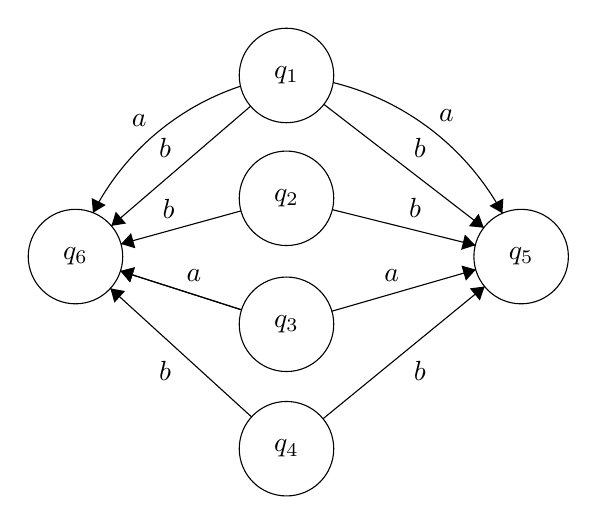
\begin{tikzpicture}[scale=0.2]
		\tikzstyle{every node}+=[inner sep=0pt]
		\draw [black] (26,-20.5) circle (3);
		\draw (26,-20.5) node {$q_2$};
		\draw [black] (26,-28.5) circle (3);
		\draw (26,-28.5) node {$q_3$};
		\draw [black] (26,-12.7) circle (3);
		\draw (26,-12.7) node {$q_1$};
		\draw [black] (26,-36.4) circle (3);
		\draw (26,-36.4) node {$q_4$};
		\draw [black] (40.9,-24.2) circle (3);
		\draw (40.9,-24.2) node {$q_5$};
		\draw [black] (12.6,-24.2) circle (3);
		\draw (12.6,-24.2) node {$q_6$};
		\draw [black] (28.962,-13.151) arc (76.21947:28.45774:16.774);
		\fill [black] (39.71,-21.45) -- (39.77,-20.51) -- (38.89,-20.98);
		\draw (36.16,-15.67) node [above] {$a$};
		\draw [black] (28.91,-21.22) -- (37.99,-23.48);
		\fill [black] (37.99,-23.48) -- (37.33,-22.8) -- (37.09,-23.77);
		\draw (34.17,-21.78) node [above] {$b$};
		\draw [black] (28.88,-27.67) -- (38.02,-25.03);
		\fill [black] (38.02,-25.03) -- (37.11,-24.77) -- (37.39,-25.73);
		\draw (32.68,-25.8) node [above] {$a$};
		\draw [black] (23.78,-34.38) -- (14.82,-26.22);
		\fill [black] (14.82,-26.22) -- (15.07,-27.13) -- (15.75,-26.39);
		\draw (18.29,-30.79) node [below] {$b$};
		\draw [black] (23.14,-27.58) -- (15.46,-25.12);
		\fill [black] (15.46,-25.12) -- (16.07,-25.84) -- (16.37,-24.88);
		\draw (20.12,-25.81) node [above] {$a$};
		\draw [black] (28.32,-34.5) -- (38.58,-26.1);
		\fill [black] (38.58,-26.1) -- (37.64,-26.22) -- (38.28,-26.99);
		\draw (34.46,-30.79) node [below] {$b$};
		\draw [black] (23.14,-27.58) -- (15.46,-25.12);
		\fill [black] (15.46,-25.12) -- (16.07,-25.84) -- (16.37,-24.88);
		\draw [black] (23.11,-21.3) -- (15.49,-23.4);
		\fill [black] (15.49,-23.4) -- (16.4,-23.67) -- (16.13,-22.71);
		\draw (18.51,-21.79) node [above] {$b$};
		\draw [black] (13.714,-21.419) arc (152.89319:108.37979:16.297);
		\fill [black] (13.71,-21.42) -- (14.52,-20.93) -- (13.63,-20.48);
		\draw (16.65,-15.99) node [above] {$a$};
		\draw [black] (23.72,-14.65) -- (14.88,-22.25);
		\fill [black] (14.88,-22.25) -- (15.81,-22.1) -- (15.16,-21.35);
		\draw (18.29,-17.96) node [above] {$b$};
		\draw [black] (28.37,-14.53) -- (38.53,-22.37);
		\fill [black] (38.53,-22.37) -- (38.2,-21.48) -- (37.59,-22.27);
		\draw (34.46,-17.95) node [above] {$b$};
	\end{tikzpicture}
\end{center}
Analogically in the example below the states also are indistinguishable but this time the outgoing transitions are the same. Hence the effects of reaching one state are equivalent to the other.

\begin{center}
	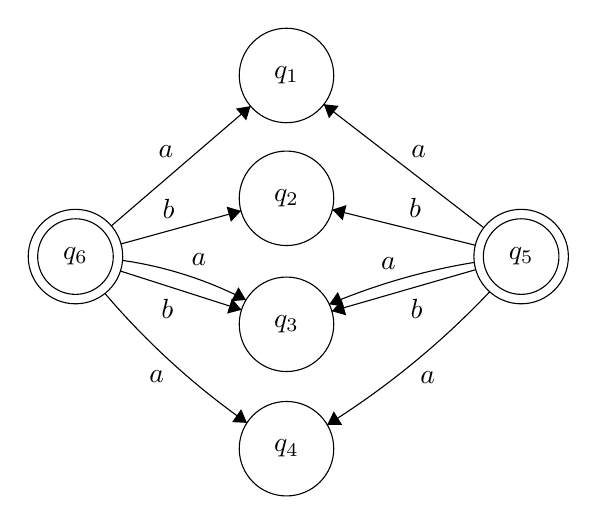
\begin{tikzpicture}[scale=0.2]
		\tikzstyle{every node}+=[inner sep=0pt]
		\draw [black] (26,-20.5) circle (3);
		\draw (26,-20.5) node {$q_2$};
		\draw [black] (26,-28.5) circle (3);
		\draw (26,-28.5) node {$q_3$};
		\draw [black] (26,-12.7) circle (3);
		\draw (26,-12.7) node {$q_1$};
		\draw [black] (26,-36.4) circle (3);
		\draw (26,-36.4) node {$q_4$};
		\draw [black] (40.9,-24.2) circle (3);
		\draw (40.9,-24.2) node {$q_5$};
		\draw [black] (40.9,-24.2) circle (2.4);
		\draw [black] (12.6,-24.2) circle (3);
		\draw (12.6,-24.2) node {$q_6$};
		\draw [black] (12.6,-24.2) circle (2.4);
		\draw [black] (14.88,-22.25) -- (23.72,-14.65);
		\fill [black] (23.72,-14.65) -- (22.79,-14.8) -- (23.44,-15.55);
		\draw (18.35,-17.96) node [above] {$a$};
		\draw [black] (15.49,-23.4) -- (23.11,-21.3);
		\fill [black] (23.11,-21.3) -- (22.2,-21.03) -- (22.47,-21.99);
		\draw (18.51,-21.79) node [above] {$b$};
		\draw [black] (15.588,-24.443) arc (81.8543:62.5633:24.571);
		\fill [black] (23.43,-26.96) -- (22.95,-26.15) -- (22.49,-27.03);
		\draw (20.44,-24.83) node [above] {$a$};
		\draw [black] (23.491,-34.756) arc (-125.02905:-139.6034:48.083);
		\fill [black] (23.49,-34.76) -- (23.12,-33.89) -- (22.55,-34.71);
		\draw (17.76,-31.42) node [below] {$a$};
		\draw [black] (38.53,-22.37) -- (28.37,-14.53);
		\fill [black] (28.37,-14.53) -- (28.7,-15.42) -- (29.31,-14.63);
		\draw (34.4,-17.95) node [above] {$a$};
		\draw [black] (37.99,-23.48) -- (28.91,-21.22);
		\fill [black] (28.91,-21.22) -- (29.57,-21.9) -- (29.81,-20.93);
		\draw (34.17,-21.78) node [above] {$b$};
		\draw [black] (28.716,-27.227) arc (112.97017:99.22512:40.045);
		\fill [black] (28.72,-27.23) -- (29.65,-27.38) -- (29.26,-26.45);
		\draw (32.47,-25.07) node [above] {$a$};
		\draw [black] (38.901,-26.436) arc (-43.42542:-57.9539:52.712);
		\fill [black] (28.59,-34.88) -- (29.53,-34.88) -- (29,-34.03);
		\draw (34.96,-31.48) node [below] {$a$};
		\draw [black] (15.46,-25.12) -- (23.14,-27.58);
		\fill [black] (23.14,-27.58) -- (22.53,-26.86) -- (22.23,-27.82);
		\draw (18.43,-26.89) node [below] {$b$};
		\draw [black] (38.02,-25.03) -- (28.88,-27.67);
		\fill [black] (28.88,-27.67) -- (29.79,-27.93) -- (29.51,-26.97);
		\draw (34.26,-26.9) node [below] {$b$};
	\end{tikzpicture}
\end{center}
The states $q_5$ and $q_6$ can be merged without affecting the language of automaton. Such a pseudo-minimisation procedure has been chosen, because it works especially well when combined with Glushkov's construction. The process of merging indistinguishable states is analogical to the process of isolating common parts of regular expression. For example the following
\[
ab+aab+ac(b+bb)
\]
could be shortened to 
\[
a(\epsilon+a+c(\epsilon+b))b
\]
by isolating the common prefix $a$ and suffix $b$. Extracting common prefixes exactly correspond to merging states with identical incoming transition, while common suffixes correspond to states with the same outgoing transitions. Sometimes there are cases that do not have any common prefix/suffix in the regular expression itself but still produce indistinguishable states in the automaton. For instance consider
\[
a+b+c+d+e
\]
which yields automaton

\begin{center}
	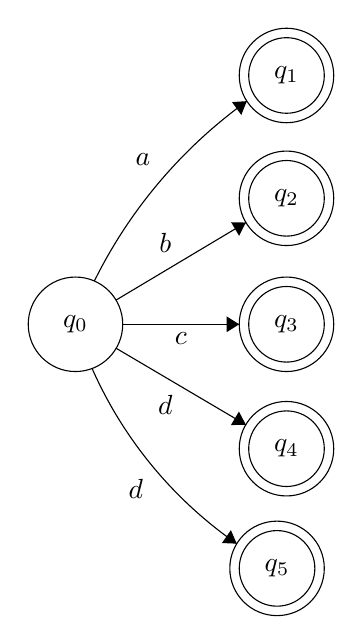
\begin{tikzpicture}[scale=0.2]
		\tikzstyle{every node}+=[inner sep=0pt]
		\draw [black] (26,-20.5) circle (3);
		\draw (26,-20.5) node {$q_2$};
		\draw [black] (26,-20.5) circle (2.4);
		\draw [black] (26,-28.5) circle (3);
		\draw (26,-28.5) node {$q_3$};
		\draw [black] (26,-28.5) circle (2.4);
		\draw [black] (26,-12.7) circle (3);
		\draw (26,-12.7) node {$q_1$};
		\draw [black] (26,-12.7) circle (2.4);
		\draw [black] (26,-36.4) circle (3);
		\draw (26,-36.4) node {$q_4$};
		\draw [black] (26,-36.4) circle (2.4);
		\draw [black] (12.6,-28.5) circle (3);
		\draw (12.6,-28.5) node {$q_0$};
		\draw [black] (25.4,-44) circle (3);
		\draw (25.4,-44) node {$q_5$};
		\draw [black] (25.4,-44) circle (2.4);
		\draw [black] (13.799,-25.751) arc (153.65447:125.74289:31.042);
		\fill [black] (23.48,-14.33) -- (22.54,-14.39) -- (23.13,-15.21);
		\draw (17.39,-18.01) node [left] {$a$};
		\draw [black] (15.18,-26.96) -- (23.42,-22.04);
		\fill [black] (23.42,-22.04) -- (22.48,-22.02) -- (22.99,-22.88);
		\draw (18.3,-24) node [above] {$b$};
		\draw [black] (15.18,-30.02) -- (23.42,-34.88);
		\fill [black] (23.42,-34.88) -- (22.98,-34.04) -- (22.47,-34.9);
		\draw (18.3,-32.95) node [below] {$d$};
		\draw [black] (15.6,-28.5) -- (23,-28.5);
		\fill [black] (23,-28.5) -- (22.2,-28) -- (22.2,-29);
		\draw (19.3,-29) node [below] {$c$};
		\draw [black] (22.844,-42.433) arc (-124.73666:-156.16311:26.641);
		\fill [black] (22.84,-42.43) -- (22.47,-41.57) -- (21.9,-42.39);
		\draw (16.93,-38.94) node [left] {$d$};
	\end{tikzpicture}
\end{center}
that could be minimised down to only two states
\begin{center}
	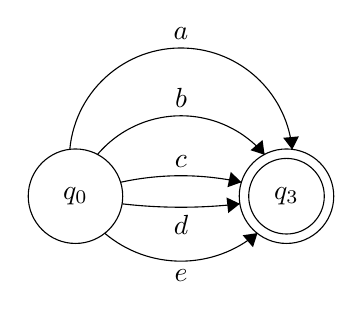
\begin{tikzpicture}[scale=0.2]
		\tikzstyle{every node}+=[inner sep=0pt]
		\draw [black] (26,-28.5) circle (3);
		\draw (26,-28.5) node {$q_3$};
		\draw [black] (26,-28.5) circle (2.4);
		\draw [black] (12.6,-28.5) circle (3);
		\draw (12.6,-28.5) node {$q_0$};
		\draw [black] (15.463,-27.615) arc (102.37767:77.62233:17.901);
		\fill [black] (23.14,-27.61) -- (22.46,-26.96) -- (22.25,-27.93);
		\draw (19.3,-26.7) node [above] {$c$};
		\draw [black] (12.238,-25.544) arc (-185.13671:-354.86329:7.091);
		\fill [black] (26.36,-25.54) -- (26.79,-24.7) -- (25.79,-24.79);
		\draw (19.3,-18.59) node [above] {$a$};
		\draw [black] (13.986,-25.865) arc (139.88963:40.11037:6.949);
		\fill [black] (24.61,-25.87) -- (24.48,-24.93) -- (23.72,-25.58);
		\draw (19.3,-22.89) node [above] {$b$};
		\draw [black] (23.04,-28.984) arc (-83.37239:-96.62761:32.407);
		\fill [black] (23.04,-28.98) -- (22.19,-28.58) -- (22.3,-29.57);
		\draw (19.3,-29.7) node [below] {$d$};
		\draw [black] (24.156,-30.841) arc (-49.67778:-130.32222:7.505);
		\fill [black] (24.16,-30.84) -- (23.22,-30.98) -- (23.87,-31.74);
		\draw (19.3,-33.12) node [below] {$e$};
	\end{tikzpicture}
\end{center}
Interestingly, the regular expression could not be minimised any further. Hence we observe that our procedure does more than a simple syntactic manipulation could achieve.

Glushkov's construction has one more advantage. Because every symbol becomes a state, it's very easy for the user to predict the exact placement of transitions between them. This way, it's easy to embed any property of the transition directly inside the regular expression. For example, suppose that we want to assign come colours to all transitions. Let $B$ stand for blue and $R$ for red. Then it's possible to embed these colours in a expression like follows
\[
aRa(Bb+Rc)R*
\]
which becomes
\[
q_1 R q_2(B q_3+R q_4)R*B
\]
We know that after $q_1$ we can read $q_2$ and along the way we have to cross the color $R$, because it stands in between $q_1$ and $q_2$. Hence it determines that the transition from $q_1$ to $q_2$ should be red. Similarly transition from $q_2$ and $q_3$ must be blue and from $q_2$ and $q_4$ is red. The transition from $q_3$ to $q_3$ will have colour $RB$, because $R$ is under the Kleen closure and $B$ is right before $q_3$. At this point we notice that there must be defined some way of mixing colours. In other words, any meta-information that we wish to embed in our regular expressions must at least form a monoid. The graph resulting from our example looks as follows

\begin{center}
	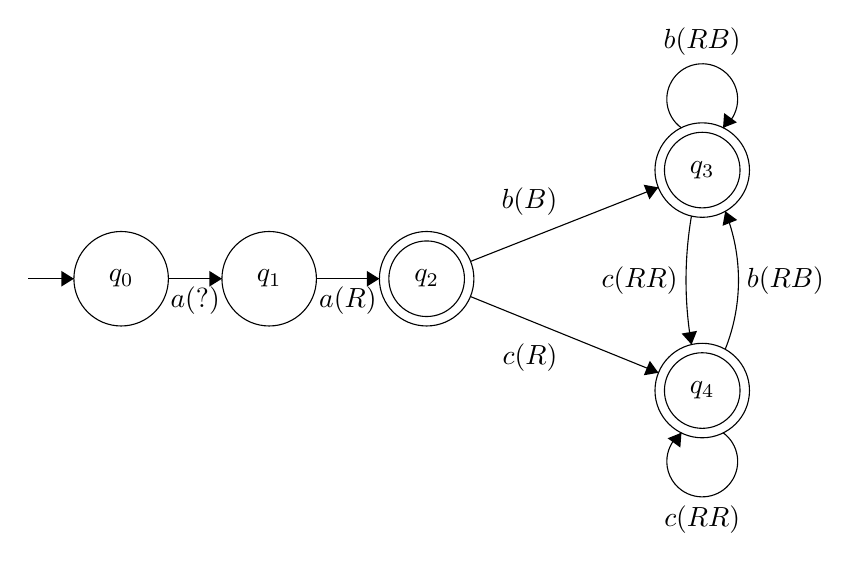
\begin{tikzpicture}[scale=0.2]
		\tikzstyle{every node}+=[inner sep=0pt]
		\draw [black] (12.6,-28.5) circle (3);
		\draw (12.6,-28.5) node {$q_0$};
		\draw [black] (22,-28.5) circle (3);
		\draw (22,-28.5) node {$q_1$};
		\draw [black] (32,-28.5) circle (3);
		\draw (32,-28.5) node {$q_2$};
		\draw [black] (32,-28.5) circle (2.4);
		\draw [black] (49.5,-21.6) circle (3);
		\draw (49.5,-21.6) node {$q_3$};
		\draw [black] (49.5,-21.6) circle (2.4);
		\draw [black] (49.5,-35.6) circle (3);
		\draw (49.5,-35.6) node {$q_4$};
		\draw [black] (49.5,-35.6) circle (2.4);
		\draw [black] (15.6,-28.5) -- (19,-28.5);
		\fill [black] (19,-28.5) -- (18.2,-28) -- (18.2,-29);
		\draw (17.3,-29) node [below] {$a(?)$};
		\draw [black] (25,-28.5) -- (29,-28.5);
		\fill [black] (29,-28.5) -- (28.2,-28) -- (28.2,-29);
		\draw (27,-29) node [below] {$a(R)$};
		\draw [black] (34.79,-27.4) -- (46.71,-22.7);
		\fill [black] (46.71,-22.7) -- (45.78,-22.53) -- (46.15,-23.46);
		\draw (38.53,-24.51) node [above] {$b(B)$};
		\draw [black] (34.78,-29.63) -- (46.72,-34.47);
		\fill [black] (46.72,-34.47) -- (46.17,-33.71) -- (45.79,-34.63);
		\draw (38.57,-32.59) node [below] {$c(R)$};
		\draw [black] (48.815,-32.681) arc (-170.33538:-189.66462:24.31);
		\fill [black] (48.82,-32.68) -- (49.17,-31.81) -- (48.19,-31.98);
		\draw (47.97,-28.6) node [left] {$c(RR)$};
		\draw [black] (50.956,-24.214) arc (21.82527:-21.82527:11.797);
		\fill [black] (50.96,-24.21) -- (50.79,-25.14) -- (51.72,-24.77);
		\draw (52.3,-28.6) node [right] {$b(RB)$};
		\draw [black] (48.177,-18.92) arc (234:-54:2.25);
		\draw (49.5,-14.35) node [above] {$b(RB)$};
		\fill [black] (50.82,-18.92) -- (51.7,-18.57) -- (50.89,-17.98);
		\draw [black] (50.823,-38.28) arc (54:-234:2.25);
		\draw (49.5,-42.85) node [below] {$c(RR)$};
		\fill [black] (48.18,-38.28) -- (47.3,-38.63) -- (48.11,-39.22);
		\draw [black] (6.7,-28.5) -- (9.6,-28.5);
		\fill [black] (9.6,-28.5) -- (8.8,-28) -- (8.8,-29);
	\end{tikzpicture}
\end{center}
Because colours form a monoid, we can use neutral element as a default value for all unspecified edges like $a(?)$. Moreover, it is also possible to attach meta-information to final states. We could imagine that an accepting state is nothing more than a state with a special outgoing transition that goes ``outside'' of automaton and has no target state. In our example the colours of such ``final'' transitions are as follows

\begin{center}
	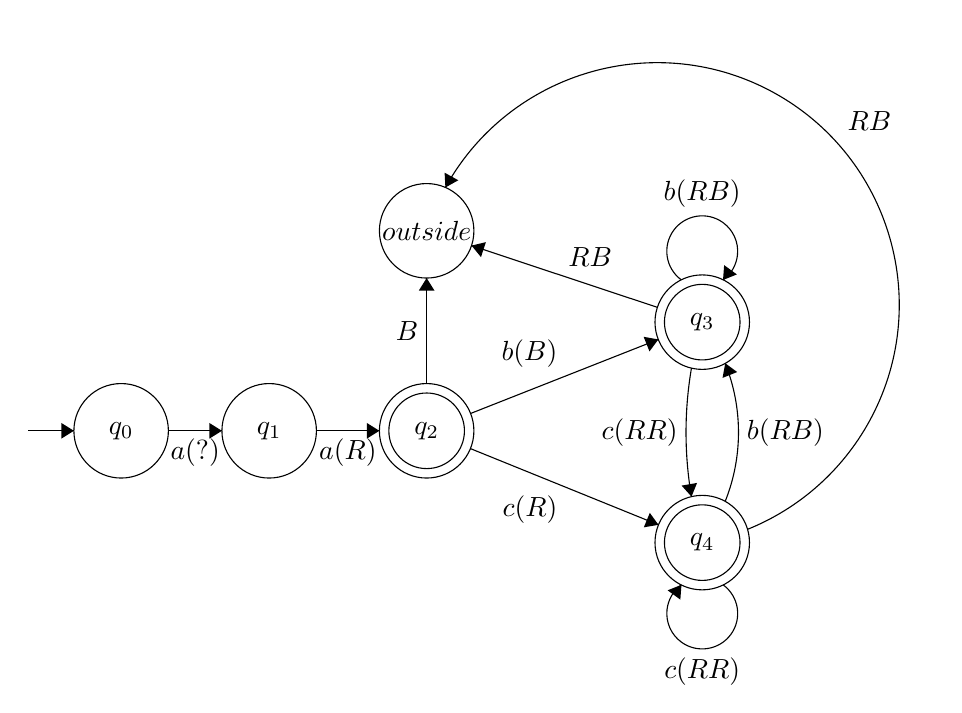
\begin{tikzpicture}[scale=0.2]
		\tikzstyle{every node}+=[inner sep=0pt]
		\draw [black] (12.6,-28.5) circle (3);
		\draw (12.6,-28.5) node {$q_0$};
		\draw [black] (22,-28.5) circle (3);
		\draw (22,-28.5) node {$q_1$};
		\draw [black] (32,-28.5) circle (3);
		\draw (32,-28.5) node {$q_2$};
		\draw [black] (32,-28.5) circle (2.4);
		\draw [black] (49.5,-21.6) circle (3);
		\draw (49.5,-21.6) node {$q_3$};
		\draw [black] (49.5,-21.6) circle (2.4);
		\draw [black] (49.5,-35.6) circle (3);
		\draw (49.5,-35.6) node {$q_4$};
		\draw [black] (49.5,-35.6) circle (2.4);
		\draw [black] (32,-15.8) circle (3);
		\draw (32,-15.8) node {$outside$};
		\draw [black] (15.6,-28.5) -- (19,-28.5);
		\fill [black] (19,-28.5) -- (18.2,-28) -- (18.2,-29);
		\draw (17.3,-29) node [below] {$a(?)$};
		\draw [black] (25,-28.5) -- (29,-28.5);
		\fill [black] (29,-28.5) -- (28.2,-28) -- (28.2,-29);
		\draw (27,-29) node [below] {$a(R)$};
		\draw [black] (34.79,-27.4) -- (46.71,-22.7);
		\fill [black] (46.71,-22.7) -- (45.78,-22.53) -- (46.15,-23.46);
		\draw (38.53,-24.51) node [above] {$b(B)$};
		\draw [black] (34.78,-29.63) -- (46.72,-34.47);
		\fill [black] (46.72,-34.47) -- (46.17,-33.71) -- (45.79,-34.63);
		\draw (38.57,-32.59) node [below] {$c(R)$};
		\draw [black] (48.815,-32.681) arc (-170.33538:-189.66462:24.31);
		\fill [black] (48.82,-32.68) -- (49.17,-31.81) -- (48.19,-31.98);
		\draw (47.97,-28.6) node [left] {$c(RR)$};
		\draw [black] (50.956,-24.214) arc (21.82527:-21.82527:11.797);
		\fill [black] (50.96,-24.21) -- (50.79,-25.14) -- (51.72,-24.77);
		\draw (52.3,-28.6) node [right] {$b(RB)$};
		\draw [black] (48.177,-18.92) arc (234:-54:2.25);
		\draw (49.5,-14.35) node [above] {$b(RB)$};
		\fill [black] (50.82,-18.92) -- (51.7,-18.57) -- (50.89,-17.98);
		\draw [black] (50.823,-38.28) arc (54:-234:2.25);
		\draw (49.5,-42.85) node [below] {$c(RR)$};
		\fill [black] (48.18,-38.28) -- (47.3,-38.63) -- (48.11,-39.22);
		\draw [black] (6.7,-28.5) -- (9.6,-28.5);
		\fill [black] (9.6,-28.5) -- (8.8,-28) -- (8.8,-29);
		\draw [black] (32,-25.5) -- (32,-18.8);
		\fill [black] (32,-18.8) -- (31.5,-19.6) -- (32.5,-19.6);
		\draw (31.5,-22.15) node [left] {$B$};
		\draw [black] (46.65,-20.66) -- (34.85,-16.74);
		\fill [black] (34.85,-16.74) -- (35.45,-17.47) -- (35.76,-16.52);
		\draw (42.38,-18.13) node [above] {$RB$};
		\draw [black] (33.189,-13.051) arc (151.02885:-68.08589:15.372);
		\fill [black] (33.19,-13.05) -- (34.01,-12.59) -- (33.14,-12.11);
		\draw (58.7,-8.86) node [right] {$RB$};
	\end{tikzpicture}
\end{center}
In Solomonoff, the meta-information of interest are transition outputs. We could imagine that strings composed of $R$ and $B$ symbols are the output of a transducer.
At this point the reader should appreciate how beautifully and naturally subsequential transducers (automata with output produced at accepting states) are derived from Glushkov's construction. As soon as we enrich regular expressions with meta-information, the state outputs emerge as if they were always there, merely hiding from the view. 

Glushkov's construction together with minimisation procedure and embedded meta-information allowed for efficient implementation of union, concatenation and Kleene closure together with output strings. In order to make the compiler applicable to real-life linguistic problems it also must support context dependent rewrites. This is a heavyweight operation that often constitutes a major performance bottleneck. Our goal was to make it as efficient as possible. 
In order to solve this issue we developed a special lexicographic semiring \cite{MendozaDrosik2020MultitapeAA}. This is an innovative solution never seen before.

Suppose we want to replace every occurrence of $abc$ with $d$. Even for such a simple scenario, the corresponding transducer will look rather complex

\begin{center}
	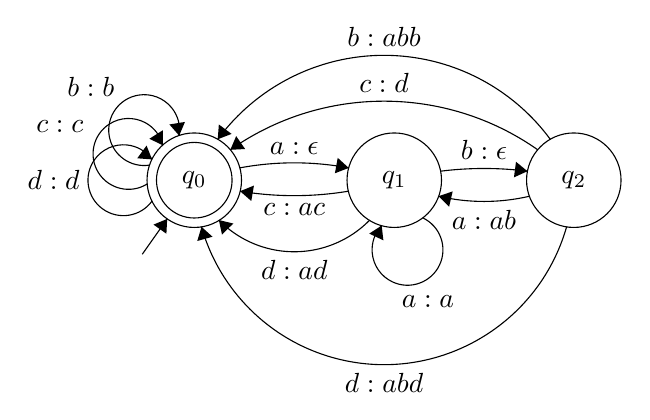
\begin{tikzpicture}[scale=0.2]
		\tikzstyle{every node}+=[inner sep=0pt]
		\draw [black] (12.6,-28.5) circle (3);
		\draw (12.6,-28.5) node {$q_0$};
		\draw [black] (12.6,-28.5) circle (2.4);
		\draw [black] (25.3,-28.5) circle (3);
		\draw (25.3,-28.5) node {$q_1$};
		\draw [black] (36.7,-28.5) circle (3);
		\draw (36.7,-28.5) node {$q_2$};
		\draw [black] (9.3,-33.2) -- (10.88,-30.96);
		\fill [black] (10.88,-30.96) -- (10.01,-31.32) -- (10.83,-31.9);
		\draw [black] (15.493,-27.717) arc (100.57485:79.42515:18.838);
		\fill [black] (22.41,-27.72) -- (21.71,-27.08) -- (21.53,-28.06);
		\draw (18.95,-26.9) node [above] {$a:\epsilon$};
		\draw [black] (28.242,-27.927) arc (97.14298:82.85702:22.176);
		\fill [black] (33.76,-27.93) -- (33.03,-27.33) -- (32.9,-28.32);
		\draw (31,-27.25) node [above] {$b:\epsilon$};
		\draw [black] (14.89,-26.568) arc (125.10167:54.89833:16.974);
		\fill [black] (14.89,-26.57) -- (15.83,-26.52) -- (15.26,-25.7);
		\draw (24.65,-22.98) node [above] {$c:d$};
		\draw [black] (9.77,-27.54) arc (279:-9:2.25);
		\draw (6.03,-23.25) node [above] {$b:b$};
		\fill [black] (11.64,-25.67) -- (12.01,-24.8) -- (11.02,-24.96);
		\draw [black] (9.621,-28.733) arc (302.19859:14.19859:2.25);
		\draw (5.59,-25.11) node [left] {$c:c$};
		\fill [black] (10.6,-26.28) -- (10.6,-25.33) -- (9.75,-25.87);
		\draw [black] (22.385,-29.199) arc (-80.6054:-99.3946:21.044);
		\fill [black] (15.51,-29.2) -- (16.22,-29.82) -- (16.39,-28.84);
		\draw (18.95,-29.98) node [below] {$c:ac$};
		\draw [black] (23.74,-31.033) arc (-44.44662:-135.55338:6.709);
		\fill [black] (14.16,-31.03) -- (14.36,-31.95) -- (15.08,-31.25);
		\draw (18.95,-33.54) node [below] {$d:ad$};
		\draw [black] (14.09,-25.904) arc (143.59719:36.40281:13.12);
		\fill [black] (14.09,-25.9) -- (14.97,-25.56) -- (14.16,-24.96);
		\draw (24.65,-20.07) node [above] {$b:abb$};
		\draw [black] (9.92,-29.823) arc (-36:-324:2.25);
		\draw (5.35,-28.5) node [left] {$d:d$};
		\fill [black] (9.92,-27.18) -- (9.57,-26.3) -- (8.98,-27.11);
		\draw [black] (36.244,-31.457) arc (-15.8876:-164.1124:12.055);
		\fill [black] (13.06,-31.46) -- (12.79,-32.36) -- (13.76,-32.09);
		\draw (24.65,-40.71) node [below] {$d:abd$};
		\draw [black] (33.885,-29.518) arc (-76.88176:-103.11824:12.713);
		\fill [black] (28.11,-29.52) -- (28.78,-30.19) -- (29.01,-29.21);
		\draw (31,-30.35) node [below] {$a:ab$};
		\draw [black] (27.1,-30.885) arc (64.76617:-223.23383:2.25);
		\draw (27.44,-35.78) node [below] {$a:a$};
		\fill [black] (24.5,-31.38) -- (23.71,-31.89) -- (24.61,-32.32);
	\end{tikzpicture}
\end{center}
A much simpler alternative would be the nondeterministic transducer

\begin{center}
	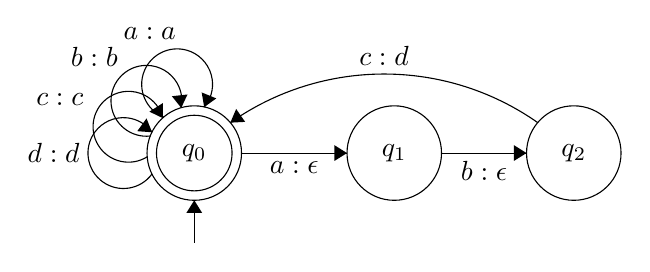
\begin{tikzpicture}[scale=0.2]
		\tikzstyle{every node}+=[inner sep=0pt]
		\draw [black] (12.6,-28.5) circle (3);
		\draw (12.6,-28.5) node {$q_0$};
		\draw [black] (12.6,-28.5) circle (2.4);
		\draw [black] (25.3,-28.5) circle (3);
		\draw (25.3,-28.5) node {$q_1$};
		\draw [black] (36.7,-28.5) circle (3);
		\draw (36.7,-28.5) node {$q_2$};
		\draw [black] (12.6,-34.2) -- (12.6,-31.5);
		\fill [black] (12.6,-31.5) -- (12.1,-32.3) -- (13.1,-32.3);
		\draw [black] (15.6,-28.5) -- (22.3,-28.5);
		\fill [black] (22.3,-28.5) -- (21.5,-28) -- (21.5,-29);
		\draw (18.95,-29) node [below] {$a:\epsilon$};
		\draw [black] (28.3,-28.5) -- (33.7,-28.5);
		\fill [black] (33.7,-28.5) -- (32.9,-28) -- (32.9,-29);
		\draw (31,-29) node [below] {$b:\epsilon$};
		\draw [black] (14.89,-26.568) arc (125.10167:54.89833:16.974);
		\fill [black] (14.89,-26.57) -- (15.83,-26.52) -- (15.26,-25.7);
		\draw (24.65,-22.98) node [above] {$c:d$};
		\draw [black] (9.815,-27.417) arc (276.48816:-11.51184:2.25);
		\draw (6.25,-23.04) node [above] {$b:b$};
		\fill [black] (11.77,-25.63) -- (12.17,-24.78) -- (11.18,-24.89);
		\draw [black] (9.621,-28.733) arc (302.19859:14.19859:2.25);
		\draw (5.59,-25.11) node [left] {$c:c$};
		\fill [black] (10.6,-26.28) -- (10.6,-25.33) -- (9.75,-25.87);
		\draw [black] (9.92,-29.823) arc (-36:-324:2.25);
		\draw (5.35,-28.5) node [left] {$d:d$};
		\fill [black] (9.92,-27.18) -- (9.57,-26.3) -- (8.98,-27.11);
		\draw [black] (10.668,-26.22) arc (248.00665:-39.99335:2.25);
		\draw (9.77,-21.33) node [above] {$a:a$};
		\fill [black] (13.23,-25.58) -- (14,-25.03) -- (13.07,-24.65);
	\end{tikzpicture}
\end{center}
The problem with such a solution is that for input strings like $aabcb$ both outputs $aabcb$ and $adb$ are generated. If only there was a way to assign priority to some outputs in order to disambiguate them, then context dependent rewrites could be expressed by much simpler automata. This is precisely what lexicographic weights are for. 

Consider the following fragment of automaton and suppose that it's possible to simultaneously nondeterministically reach both $q_2$ and $q_1$.
\begin{center}
	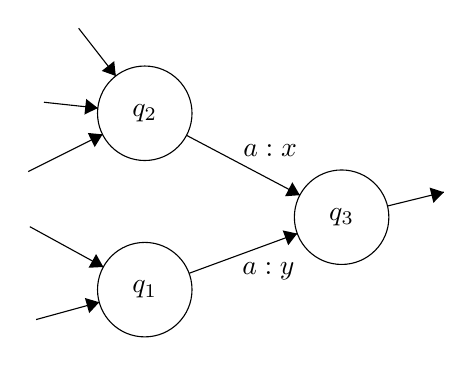
\begin{tikzpicture}[scale=0.2]
		\tikzstyle{every node}+=[inner sep=0pt]
		\draw [black] (24.2,-33.1) circle (3);
		\draw (24.2,-33.1) node {$q_1$};
		\draw [black] (36.7,-28.5) circle (3);
		\draw (36.7,-28.5) node {$q_3$};
		\draw [black] (24.2,-21.9) circle (3);
		\draw (24.2,-21.9) node {$q_2$};
		\draw [black] (27.02,-32.06) -- (33.88,-29.54);
		\fill [black] (33.88,-29.54) -- (32.96,-29.34) -- (33.31,-30.28);
		\draw (32.05,-31.34) node [below] {$a:y$};
		\draw [black] (26.85,-23.3) -- (34.05,-27.1);
		\fill [black] (34.05,-27.1) -- (33.57,-26.28) -- (33.11,-27.17);
		\draw (32.16,-24.69) node [above] {$a:x$};
		\draw [black] (16.8,-25.6) -- (21.52,-23.24);
		\fill [black] (21.52,-23.24) -- (20.58,-23.15) -- (21.02,-24.05);
		\draw [black] (16.9,-29.1) -- (21.57,-31.66);
		\fill [black] (21.57,-31.66) -- (21.11,-30.84) -- (20.63,-31.71);
		\draw [black] (17.3,-35) -- (21.31,-33.9);
		\fill [black] (21.31,-33.9) -- (20.4,-33.63) -- (20.67,-34.59);
		\draw [black] (17.8,-21.2) -- (21.22,-21.57);
		\fill [black] (21.22,-21.57) -- (20.48,-20.99) -- (20.37,-21.98);
		\draw [black] (20,-16.5) -- (22.36,-19.53);
		\fill [black] (22.36,-19.53) -- (22.26,-18.59) -- (21.47,-19.21);
		\draw [black] (39.61,-27.79) -- (43.19,-26.91);
		\fill [black] (43.19,-26.91) -- (42.29,-26.62) -- (42.53,-27.59);
	\end{tikzpicture}
\end{center}
If the next input symbol is $a$, then the transducer will reach state $q_3$ and generate two outputs --- one ending in $x$ and the other in $y$. If the automaton later accepts it will produce at least two ambiguous outputs.
Lexicographic weights allow us to assign priority to different transitions.
In the following example, only the output ending in $x$ will reach state $q_3$ and the other ending in $y$ will be discarded because it came to $q_3$ over transition with lower weight.
\begin{center}
	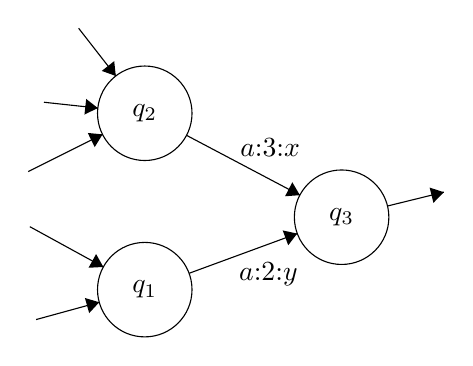
\begin{tikzpicture}[scale=0.2]
		\tikzstyle{every node}+=[inner sep=0pt]
		\draw [black] (24.2,-33.1) circle (3);
		\draw (24.2,-33.1) node {$q_1$};
		\draw [black] (36.7,-28.5) circle (3);
		\draw (36.7,-28.5) node {$q_3$};
		\draw [black] (24.2,-21.9) circle (3);
		\draw (24.2,-21.9) node {$q_2$};
		\draw [black] (27.02,-32.06) -- (33.88,-29.54);
		\fill [black] (33.88,-29.54) -- (32.96,-29.34) -- (33.31,-30.28);
		\draw (32.05,-31.34) node [below] {$a{:}2{:}y$};
		\draw [black] (26.85,-23.3) -- (34.05,-27.1);
		\fill [black] (34.05,-27.1) -- (33.57,-26.28) -- (33.11,-27.17);
		\draw (32.16,-24.69) node [above] {$a{:}3{:}x$};
		\draw [black] (16.8,-25.6) -- (21.52,-23.24);
		\fill [black] (21.52,-23.24) -- (20.58,-23.15) -- (21.02,-24.05);
		\draw [black] (16.9,-29.1) -- (21.57,-31.66);
		\fill [black] (21.57,-31.66) -- (21.11,-30.84) -- (20.63,-31.71);
		\draw [black] (17.3,-35) -- (21.31,-33.9);
		\fill [black] (21.31,-33.9) -- (20.4,-33.63) -- (20.67,-34.59);
		\draw [black] (17.8,-21.2) -- (21.22,-21.57);
		\fill [black] (21.22,-21.57) -- (20.48,-20.99) -- (20.37,-21.98);
		\draw [black] (20,-16.5) -- (22.36,-19.53);
		\fill [black] (22.36,-19.53) -- (22.26,-18.59) -- (21.47,-19.21);
		\draw [black] (39.61,-27.79) -- (43.19,-26.91);
		\fill [black] (43.19,-26.91) -- (42.29,-26.62) -- (42.53,-27.59);
	\end{tikzpicture}
\end{center}
Lexicographic weights allow to make the transducers even more compact. We proved that there exist weighted automata exponentially smaller than even the smallest unweighted nondeterministic ones. In the presence of lexicographic weights, context-dependent rewrites become expressible directly in Glushkov's construction, without the need for calling any ``external operations''. 

In the tasks of natural language processing it's common to work with large alphabets. User input might contain unexpected sequences like math symbols, foreign words or even emojis and other UNICODE entities. The regular expressions should handle such cases gracefully, especially when using wildcards such as \texttt{.*} or \texttt{\textbackslash p\{Lu\}}. Representation of large character classes is a challenging task for finite state automata. In order to use the dot wildcard in UNICODE, the automaton would require millions of transitions, one for each individual symbol. 
In order to optimise this, Solomonoff employs symbolic transitions \cite{symbolic_transducers}. While classic automata have edges labelled with individual symbols, our transducers have edges that span entire ranges. A range is easy to encode in computer memory. It's enough to store the first and last symbol. Below is an example of classical finite state automaton

\begin{center}
	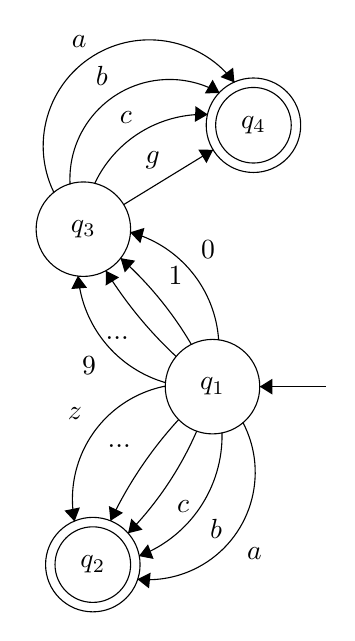
\begin{tikzpicture}[scale=0.2]
		\tikzstyle{every node}+=[inner sep=0pt]
		\draw [black] (21.9,-33.8) circle (3);
		\draw (21.9,-33.8) node {$q_1$};
		\draw [black] (14.3,-45.1) circle (3);
		\draw (14.3,-45.1) node {$q_2$};
		\draw [black] (14.3,-45.1) circle (2.4);
		\draw [black] (13.7,-23.8) circle (3);
		\draw (13.7,-23.8) node {$q_3$};
		\draw [black] (24.5,-17.2) circle (3);
		\draw (24.5,-17.2) node {$q_4$};
		\draw [black] (24.5,-17.2) circle (2.4);
		\draw [black] (29.1,-33.8) -- (24.9,-33.8);
		\fill [black] (24.9,-33.8) -- (25.7,-34.3) -- (25.7,-33.3);
		\draw [black] (23.827,-36.068) arc (27.74974:-95.59664:6.819);
		\fill [black] (17.13,-46.03) -- (17.87,-46.61) -- (17.97,-45.61);
		\draw (24.06,-44.39) node [right] {$a$};
		\draw [black] (22.505,-36.721) arc (1.21842:-69.06533:8.204);
		\fill [black] (17.23,-44.56) -- (18.16,-44.74) -- (17.8,-43.81);
		\draw (21.72,-42.81) node [right] {$b$};
		\draw [black] (20.897,-36.625) arc (-23.51659:-44.33031:21.62);
		\fill [black] (16.54,-43.11) -- (17.46,-42.88) -- (16.74,-42.18);
		\draw (19.62,-41.4) node [right] {$c$};
		\draw [black] (15.425,-42.321) arc (154.65938:137.49372:25.965);
		\fill [black] (15.42,-42.32) -- (16.22,-41.81) -- (15.32,-41.38);
		\draw (16.74,-37.6) node [left] {$...$};
		\draw [black] (13.142,-42.355) arc (-168.87:-258.9769:7.316);
		\fill [black] (13.14,-42.36) -- (13.48,-41.47) -- (12.5,-41.67);
		\draw (13.64,-35.52) node [left] {$z$};
		\draw [black] (16.674,-23.995) arc (74.9508:3.75271:7.609);
		\fill [black] (16.67,-24) -- (17.32,-24.69) -- (17.58,-23.72);
		\draw (21.14,-25.09) node [right] {$0$};
		\draw [black] (16.065,-25.642) arc (48.30476:30.39874:22.759);
		\fill [black] (16.06,-25.64) -- (16.33,-26.55) -- (16.99,-25.8);
		\draw (19.08,-26.77) node [right] {$1$};
		\draw [black] (19.593,-31.885) arc (-132.96338:-148.33311:26.34);
		\fill [black] (15.13,-26.44) -- (15.12,-27.38) -- (15.97,-26.86);
		\draw (16.62,-30.74) node [left] {$...$};
		\draw [black] (18.929,-33.549) arc (-105.96776:-175.32874:7.713);
		\fill [black] (13.36,-26.76) -- (12.93,-27.6) -- (13.93,-27.52);
		\draw (14.53,-32.46) node [left] {$9$};
		\draw [black] (11.835,-21.482) arc (-153.92109:-323.21978:6.741);
		\fill [black] (23.29,-14.48) -- (23.21,-13.54) -- (22.41,-14.14);
		\draw (13.43,-12.27) node [above] {$a$};
		\draw [black] (12.853,-20.951) arc (-177.02573:-300.11514:6.33);
		\fill [black] (22.35,-15.15) -- (21.91,-14.31) -- (21.41,-15.18);
		\draw (14.87,-14.72) node [above] {$b$};
		\draw [black] (14.415,-20.906) arc (154.87614:87.98299:7.638);
		\fill [black] (21.6,-16.52) -- (20.82,-15.99) -- (20.78,-16.99);
		\draw (16.4,-17.13) node [above] {$c$};
		\draw [black] (16.26,-22.24) -- (21.94,-18.76);
		\fill [black] (21.94,-18.76) -- (21,-18.75) -- (21.52,-19.61);
		\draw (18.1,-20) node [above] {$g$};
	\end{tikzpicture}
\end{center}
and an equivalent symbolic automaton that uses closed ranges of symbols as transition predicates
\begin{center}
	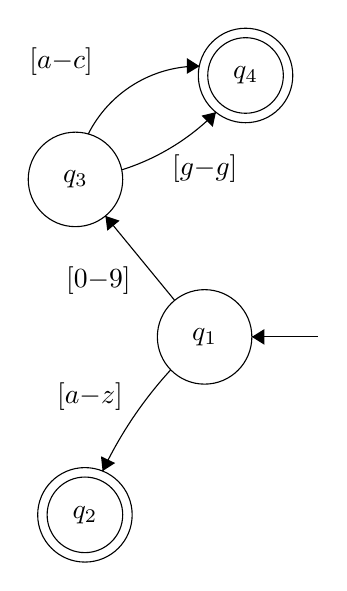
\begin{tikzpicture}[scale=0.2]
		\tikzstyle{every node}+=[inner sep=0pt]
		\draw [black] (21.9,-33.8) circle (3);
		\draw (21.9,-33.8) node {$q_1$};
		\draw [black] (14.3,-45.1) circle (3);
		\draw (14.3,-45.1) node {$q_2$};
		\draw [black] (14.3,-45.1) circle (2.4);
		\draw [black] (13.7,-23.8) circle (3);
		\draw (13.7,-23.8) node {$q_3$};
		\draw [black] (24.5,-17.2) circle (3);
		\draw (24.5,-17.2) node {$q_4$};
		\draw [black] (24.5,-17.2) circle (2.4);
		\draw [black] (29.1,-33.8) -- (24.9,-33.8);
		\fill [black] (24.9,-33.8) -- (25.7,-34.3) -- (25.7,-33.3);
		\draw [black] (15.425,-42.321) arc (154.65938:137.49372:25.965);
		\fill [black] (15.42,-42.32) -- (16.22,-41.81) -- (15.32,-41.38);
		\draw (16.74,-37.6) node [left] {$[a {-} z]$};
		\draw [black] (20,-31.48) -- (15.6,-26.12);
		\fill [black] (15.6,-26.12) -- (15.72,-27.06) -- (16.5,-26.42);
		\draw (17.24,-30.23) node [left] {$[0{-}9]$};
		\draw [black] (14.506,-20.929) arc (153.34454:89.5146:7.838);
		\fill [black] (21.58,-16.61) -- (20.78,-16.1) -- (20.77,-17.1);
		\draw (12.79,-17.25) node [above] {$[a{-}c]$};
		\draw [black] (22.625,-19.535) arc (-44.65667:-72.4842:14.6);
		\fill [black] (22.62,-19.53) -- (21.71,-19.75) -- (22.42,-20.46);
		\draw (21.91,-22.23) node [below] {$[g{-}g]$};
	\end{tikzpicture}
\end{center}
Compilation of transducers is the core part of our library but in order to make the automata useful there must be a way to execute them. Deterministic transducers and Mealy machines could be evaluated in linear time. Nondeterministic automata are more expensive. The computation might branch and the automaton could be in multiple states simultaneously. Using dynamic programming it's possible to build a table with rows representing consecutive symbols of input string and each column keeping track of one state. 
At each step of execution, one input symbol is read and one row in the table is filled based on the contents of the previous row. Below is an example of nondeterministic finite state automaton and its corresponding evaluation table after reading input string $aba$.

\begin{center}
	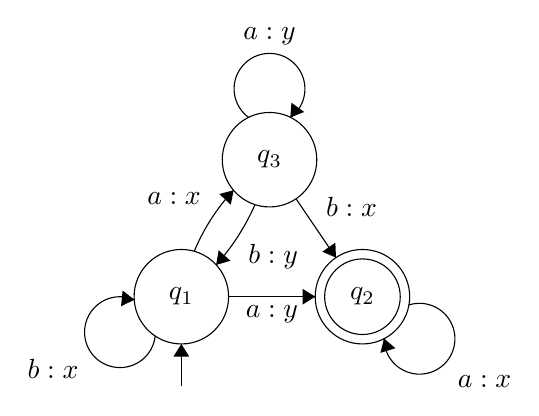
\begin{tikzpicture}[scale=0.2]
		\tikzstyle{every node}+=[inner sep=0pt]
		\draw [black] (16.5,-23.2) circle (3);
		\draw (16.5,-23.2) node {$q_1$};
		\draw [black] (28,-23.2) circle (3);
		\draw (28,-23.2) node {$q_2$};
		\draw [black] (28,-23.2) circle (2.4);
		\draw [black] (22.1,-14.5) circle (3);
		\draw (22.1,-14.5) node {$q_3$};
		\draw [black] (19.5,-23.2) -- (25,-23.2);
		\fill [black] (25,-23.2) -- (24.2,-22.7) -- (24.2,-23.7);
		\draw (22.25,-23.7) node [below] {$a:y$};
		\draw [black] (17.318,-20.321) arc (157.50332:136.95968:12.951);
		\fill [black] (19.82,-16.44) -- (18.91,-16.68) -- (19.64,-17.36);
		\draw (17.77,-16.95) node [left] {$a:x$};
		\draw [black] (23.78,-16.98) -- (26.32,-20.72);
		\fill [black] (26.32,-20.72) -- (26.28,-19.77) -- (25.45,-20.34);
		\draw (25.66,-17.5) node [right] {$b:x$};
		\draw [black] (21.18,-17.35) arc (-23.77693:-41.76007:14.582);
		\fill [black] (18.71,-21.18) -- (19.62,-20.92) -- (18.87,-20.25);
		\draw (20.72,-20.68) node [right] {$b:y$};
		\draw [black] (20.777,-11.82) arc (234:-54:2.25);
		\draw (22.1,-7.25) node [above] {$a:y$};
		\fill [black] (23.42,-11.82) -- (24.3,-11.47) -- (23.49,-10.88);
		\draw [black] (30.942,-23.725) arc (107.61565:-180.38435:2.25);
		\draw (34.02,-28.59) node [right] {$a:x$};
		\fill [black] (29.37,-25.85) -- (29.14,-26.77) -- (30.09,-26.47);
		\draw [black] (14.841,-25.685) arc (-5.99178:-293.99178:2.25);
		\draw (10,-27.81) node [left] {$b:x$};
		\fill [black] (13.52,-23.39) -- (12.77,-22.81) -- (12.67,-23.81);
		\draw [black] (16.5,-28.9) -- (16.5,-26.2);
		\fill [black] (16.5,-26.2) -- (16,-27) -- (17,-27);
	\end{tikzpicture}
\end{center}

\begin{table}[!htbp]
	\centering
	\begin{tabular}{|l|l|l|l|}
		\hline
		symbol                                                          & $q_1$ & $q_2$ & $q_3$ \\ \hline
		\begin{tabular}[c]{@{}l@{}}initial\\ configuration\end{tabular} & 1    & 0    & 0    \\ \hline
		a                                                               & 0    & 1    & 1    \\ \hline
		b                                                               & 1    & 1    & 0    \\ \hline
		a                                                               & 0    & 1    & 1    \\ \hline
	\end{tabular}
\end{table}

By the end of evaluating such a table, it's enough to scan the last row to find a column of some accepting state. In the above example, such a state is $q_2$ and we can observe that it's active in the last row.

In case of transducers, we not only want to know, whether the string was accepted or not but also the output generated along the way. In order to do this  the table can be backtracked from the accepting state backwards. For the backtracking step to be possible, we need to store information about the source state of each taken transition. 

\begin{table}[!htbp]
	\centering
	\begin{tabular}{|l|l|l|l|}
		\hline
		symbol                                                          & $q_1$ & $q_2$ & $q_3$ \\ \hline
		\begin{tabular}[c]{@{}l@{}}initial\\ configuration\end{tabular} & $q_1$    & $\emptyset$    & $\emptyset$    \\ \hline
		a                                                               & $\emptyset$    & $q_1$    & $q_1$    \\ \hline
		b                                                               & $q_3$    & $q_3$    & $\emptyset$    \\ \hline
		a                                                               & $\emptyset$    & $q_1$    & $q_1$    \\ \hline
	\end{tabular}
\end{table}
Assuming that every transition is uniquely determined by its symbol, source state and target state (in other words $\delta:Q\times \Sigma\times Q \rightarrow \Gamma^*$), it becomes possible to use such an evaluation table to find the exact accepting path in automaton and collect all the outputs printed along the way. 

This algorithm has been made even more efficient by using techniques from graph theory. Every automaton is a directed graph that could be represented as an adjacency matrix \cite{graphTheory}. An example is shown below.
\begin{table}[!htbp]
	\centering
	\begin{tabular}{|l|l|l|l|}
		\hline
		adjacency & $q_1$      & $q_2$ & $q_3$      \\ \hline
		$q_1$     & b:x        & a:y   & a:x        \\ \hline
		$q_2$     & $\emptyset$ & a:x   & $\emptyset$ \\ \hline
		$q_3$     & b:y        & b:x   & a:y        \\ \hline
	\end{tabular}
\end{table}

Sparse graphs can be optimised and instead of using matrix it's possible to only store the list of adjacent vertices. 
\[
(q_1,b:x,q_1), (q_1,a:y,q_2), (q_1,a:x,q_3), (q_2,a:x,q_2), (q_3,b:y,q_3), ...
\]
Nondeterministic  automata very often are the perfect example of sparse graphs. Hence instead of using an evaluation table, it's better to use a list of states nondeterministically reached at any given step of evaluation. 
\begin{table}[!htbp]
	\centering
	\begin{tabular}{|l|l|}
		\hline
		symbol                                                          & list \\ \hline
		\begin{tabular}[c]{@{}l@{}}initial\\ configuration\end{tabular} & $q_1$ \\ \hline
		a                                                               & $q_2,q_3$    \\ \hline
		b                                                               & $q_1,q_2$    \\ \hline
		a                                                               & $q_2,q_3$    \\ \hline
	\end{tabular}
\end{table}

The backtracking can be made efficient by storing pointer to the source state of any taken transition.

\begin{table}[!htbp]
	\centering
	\begin{tabular}{|l|l|}
		\hline
		symbol                                                          & list \\ \hline
		\begin{tabular}[c]{@{}l@{}}initial\\ configuration\end{tabular} & $q_1(\mbox{ from }q_1)$ \\ \hline
		a                                                               & $q_2(\mbox{ from }q_1), q_3(\mbox{ from }q_1)$    \\ \hline
		b                                                               & $ q_1(\mbox{ from }q_3), q_2(\mbox{ from }q_3)$    \\ \hline
		a                                                               & $q_2(\mbox{ from }q_1),  q_3(\mbox{ from }q_1)$    \\ \hline
	\end{tabular}
\end{table}

Glushkov's construction relies on building three sets: the set of initial symbols, final symbols and 2-factor \cite{GLUSHKOV} strings (that is, all substrings of length 2). The early prototype versions of Solomonoff would represent sets as bitsets, where each bit specifies whether an element belongs to the set or not. This representation simplified implementation of many algorithms but was highly inefficient. Later implementation used hash sets instead. While hash maps have constant insertions and deletions, they ensure it at the cost of larger memory consumption. During benchmarks on real-life datasets, Solomonoff would often run out of memory and crash.  The final version uses signly linkged graphs backed by arrays. This provides the highest efficiency with the smallest memory footprint but it is non-trivial to implement. The optimisation relies on representing sparse sets as arrays of elements. This approach proved to be the best choice, because Glushkov's construction inherently ensures uniqueness of all inserted elements (hence using hashes to search for duplicates before insertion was not necessary)  and it does not use deletions. As a result any array was guaranteed to behave like a set.

The standard definition of Glushkov's construction produces a set of 2-factors as its output. Then a separate procedure would be necessary to collect all such strings and convert them into a graph of automaton. We found a way to make it more efficient and build the graph directly. The step of building 2-factors was entirely bypassed. This provided even further optimisation.

One of the core features of Solomonoff is the algorithm for detecting ambiguous nondeterminism. Advance-and-delay procedure can check functionality of automaton in quadratic time. While the compiler does provide implementation of this procedure, it is not used for checking functionality. Instead we use a simpler algorithm for checking strong functionality of lexicographic weights \cite{MendozaDrosik2020MultitapeAA}. While the performance difference between the two is negligable, the advantage of our approach comes from  better error messages in case of nondeterminism. If some lexicographic weights are in conflict with each other, the compiler can point the user to the exact line and column of text where the conflict arises, whereas advance-and-delay might miss the origin of the problem and only fail further down the line.

\section{Gluszkov's construction}


In this section we provide formal and mathematically rigorous presentation of Glushkov's construction. 

The theory of automata is primarily founded on the theory of semigroups and monoids. A set $X$ together with operation $\oplus:X\times X \rightarrow X$ forms a semigroup if it satisfies associativity $(x_1 \oplus x_2) \oplus x_3= x_1 \oplus (x_2 \oplus x_3)$. If the semigroup contains a neutral element $0_X$ such that $0_X \oplus x = x \oplus 0_X = 0_X$ then it forms a monoid. For example the set of positive (zero excluded) integers together with addition operation forms a semigroup, while a set of non-negative integers (zero included) forms a monoid. Because of associativity, the placement of brackets does not matter and can be omitted  altogether. As a result instead of writing 
\[
((x_1\oplus (x_2 \oplus x_3)) \oplus x_4)\oplus (x_5\oplus x_6)
\]
we can just write 
\[
x_1 x_2  x_3 x_4 x_5 x_6
\]
Every element of $X$ can be presented in such a way.  String of elements of $X$ connected together with the operation $\oplus$ is called a word. There might be more than one word denoting the same element. For example, the number $6$ could be framed as $0+1+2+3$ or $0+6+0$ or just $6$. All of those are different words denoting the same number. A free semigroup is one in which no two distinct words denote the same element. The canonical example of free semigroup is the set of all non-empty strings under concatenation. No two strings are equal, unless their notations are syntactically the same. Definition of free monoid is similar to free semigroup, with the exception that neutral elements do not change denotation of a word. For example the following words must all be equal $0+3+4=3+0+4=3+4+0+0$ but all of $4+3 \ne 3+4 \ne 1+1+1+4 \ne 1 + 5 + 1$ must be different from each other. The standard example of free monoid is the set of all strings with concatenation operation. No two strings are equal, except for the ones that are concatenated with the empty string $\epsilon$. 

Given two monoids $X$ and $Y$ with operations $\oplus$ and $\odot$ respectively, it's possible to build a new one by performing their direct product $X \times Y$. Their joint operation is defined as $(x_1,y_1)\cdot(x_2,y_2) = (x_1 \oplus x_2, y_1 \odot y2)$.


Let $\Sigma$ be the (not necessarily finite) alphabet of automaton. Let $\chi$ be the set of subsets of $\Sigma$ that we will call ranges of $\Sigma$. Let  $\overline{\chi}$ be  the closure of $\chi$ under countable union and complementation (so it forms a sigma algebra). For instance, imagine that there is a total order on $\Sigma$ and  $\chi$ is the set of all intervals in $\Sigma$. Now we want to build an automaton whose transitions are not labelled with symbols from $\Sigma$, but rather with ranges from $\chi$. Union $\chi_0\cup\chi_1$ of two elements from $\chi$ ``semantically'' corresponds to putting two edges, $(q,\chi_0,q')\in\delta$ (for a moment forget about outputs and weights) and $(q,\chi_1,q')\in\delta$. There is no limitation on the size of $\delta$. It might be countably infinite, hence it's natural that $\overline{\chi}$ should be closed under countable union. Therefore, $\chi$ is the set of allowed transition labels and $\overline{\chi}$ is the set of all possible ``semantic'' transitions. We could say that $\overline{\chi}$ is discrete if it contains every subset of $\Sigma$. An example of discrete $\overline{\chi}$ would be a finite set $\Sigma$ with all UNIX-style ranges \texttt{[$\sigma$-$\sigma'$]} included in $\chi$. 

Transducers with input $\Sigma^*$ and output $\Gamma^*$ can be seen as a finite state automaton working with single input $\Sigma^* \times \Gamma^*$. Therefore we can treat every pair of symbols $(\sigma,\gamma)$ as an atomic formula of regular expressions for transducers. We can use concatenation $(\sigma,\gamma_0)(\epsilon,\gamma_1)$ to represent $(\sigma,\gamma_0\gamma_1)$. It's possible to create ambiguous transducers with unions like  $(\epsilon,\gamma_0)+(\epsilon,\gamma_1)$.  To make notation easier, we will treat every $\sigma$ as $(\sigma,\epsilon)$ and every $\gamma$ as $(\epsilon,\gamma)$. Then instead of writing lengthy $(\sigma,\epsilon)(\epsilon,\gamma)$ we could introduce shortened notation $\sigma:\gamma$. Because we would like to avoid ambiguous transducers we can put restriction that the right side of $:$ should always be a string of $\Gamma^*$ and writing entire formulas (like $\sigma:\gamma_1+\gamma_2^*$) is not allowed. This restriction will later simplify Glushkov's algorithm. 

We define $\mathcal{A}^\Sigma$ to be the set of atomic characters. For instance we could choose $\mathcal{A}^\Sigma=\Sigma\cup\{\epsilon\}$ for FSA/transducers and $\mathcal{A}^\Sigma=\chi$ for ranged automata. 

We call  $RE^{\Sigma:D}$ the set of all regular expression formulas with the underlying set of atomic characters $\mathcal{A}^\Sigma$ and allowed output strings $D$. It's possible that $D$ might be a singleton monoid $\{\epsilon \}$ but it should not be empty, because then no element would belong to $\Sigma^* \times D$. By inductive definition, if $\phi$ and $\psi$  are $RE^{ \Sigma:D}$  formulas and $d \in D$, then union $\phi + \psi$, concatenation $\phi \cdot \psi$, Kleene closure $\phi^*$ and output concatenation $\phi : d$ are $RE^{ \Sigma:D}$ formulas as well.  Define $V^{\Sigma:D}:RE^{\Sigma:D} \rightarrow \Sigma^* \times D$ to be the valuation function:  \\
$V^{\Sigma:D}(\phi + \psi) = V^{\Sigma:D}(\phi) \cup V^{\Sigma:D}(\psi)$ \\
$V^{\Sigma:D}(\phi \cdot \psi) = V^{\Sigma:D}(\phi) \cdot  V^{\Sigma:D}(\psi)$ \\
$V^{\Sigma:D}(\phi^*) = (\epsilon,\epsilon) + V^{\Sigma:D}(\phi) + V^{\Sigma:D}(\phi)^2 + ...$ \\
$V^{\Sigma:D}(\phi : d) = V^{\Sigma:D}(\phi)  \cdot (\epsilon,d)$ \\
$V^{\Sigma:D}(a) = a$ where $a\in\mathcal{A}^{\Sigma:D}$ \\
Some notable properties are: \\
$x:y_0 +x:y_1 = x:(y_0+y_1)$ \\
$x:\epsilon+x:y+x:y^2...=x:y^*$ \\
$(x:y_0)(\epsilon:y_1)  = x:(y_0y_1)$\\
$x_0:(y_0y')+x_1:(y_1y') = (x_0:y_0+x_1:y1)\cdot(\epsilon:y')$ \\
$x_0:(y'y_0)+x_1:(y'y_1) = (\epsilon:y')\cdot(x_0:y_0+x_1:y1)$  \\
Therefore we can see that expressive power with and without $:$ is the same. 

It's also possible to extend regular expressions with weights. Let $RE_W^{\Sigma: D}$ be a superset of $RE^{\Sigma: D}$ and $W$ be the set of weight symbols. If $\phi\in RE_W^{\Sigma\rightarrow D}$ and $w_0,w_1\in W$ then $w_0 \phi $ and  $\phi w_1 $ are in $RE_W^{\Sigma\rightarrow D}$. This allows for inserting weight at any place. For instance, the automaton below

\begin{center}
	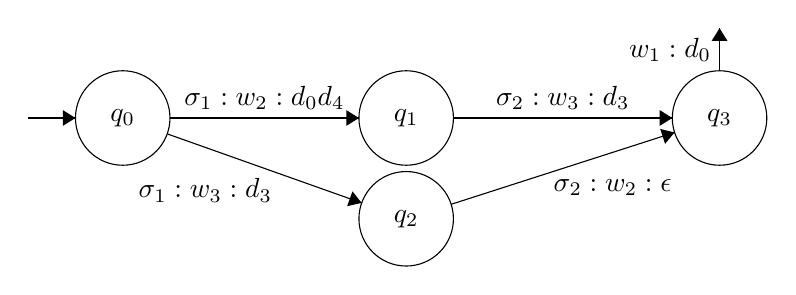
\begin{tikzpicture}[scale=0.2]
		\tikzstyle{every node}+=[inner sep=0pt]
		\draw [black] (18.5,-26.2) circle (3);
		\draw (18.5,-26.2) node {$q_0$};
		\draw [black] (36.5,-26.2) circle (3);
		\draw (36.5,-26.2) node {$q_1$};
		\draw [black] (56.4,-26.2) circle (3);
		\draw (56.4,-26.2) node {$q_3$};
		\draw [black] (36.5,-32.6) circle (3);
		\draw (36.5,-32.6) node {$q_2$};
		\draw [black] (21.5,-26.2) -- (33.5,-26.2);
		\fill [black] (33.5,-26.2) -- (32.7,-25.7) -- (32.7,-26.7);
		\draw (27.5,-25.7) node [above] {$\sigma_1:w_2:d_0d_4$};
		\draw [black] (39.5,-26.2) -- (53.4,-26.2);
		\fill [black] (53.4,-26.2) -- (52.6,-25.7) -- (52.6,-26.7);
		\draw (46.45,-25.7) node [above] {$\sigma_2:w_3:d_3$};
		\draw [black] (21.33,-27.21) -- (33.67,-31.59);
		\fill [black] (33.67,-31.59) -- (33.09,-30.86) -- (32.75,-31.8);
		\draw (23.74,-30.02) node [below] {$\sigma_1:w_3:d_3$};
		\draw [black] (39.36,-31.68) -- (53.54,-27.12);
		\fill [black] (53.54,-27.12) -- (52.63,-26.89) -- (52.94,-27.84);
		\draw (49.61,-30.05) node [below] {$\sigma_2:w_2:\epsilon$};
		\draw [black] (56.4,-23.2) -- (56.4,-20.5);
		\fill [black] (56.4,-20.5) -- (55.9,-21.3) -- (56.9,-21.3);
		\draw (55.9,-21.85) node [left] {$w_1:d_0$};
		\draw [black] (12.5,-26.2) -- (15.5,-26.2);
		\fill [black] (15.5,-26.2) -- (14.7,-25.7) -- (14.7,-26.7);
	\end{tikzpicture}
\end{center}
could be expressed using \[
((\sigma_1:d_0d_4)w_2(\sigma_2:d_3)w_3+
(\sigma_1:d_3)w_3\sigma_2w_2):d_0
\]
The definition of $V^{\Sigma:D}(\phi w)$ depends largely on $W$ but associativity $(\phi w_1) w_2 = \phi (w_1 + w_2)$ should be preserved, given that $W$ is an additive monoid. This also implies that $w_1 \epsilon w_2 = w_1 w_2$, which is semantically equivalent to the addition $w_1 + w_2$. 


First step of Glushkov's algorithm is to create a new alphabet $\Omega$ in which every atomic character (including duplicates but excluding $\epsilon$) in $\phi$ is treated as a new individual character. As a result we should obtain new rewritten formula 
$\psi \in RE_W^{\Omega \rightarrow D} $ along with mapping $\alpha:\Omega \rightarrow\mathcal{A}^\Sigma$. This mapping will remember the original atomic character, before it was rewritten to a unique symbol in $\Omega$.
For example 
\[
\phi=(\epsilon:x_0) x_0(x_0:x_1x_3)x_3 w_0+(x_1x_2)^* w_1
\]
will be rewritten as 
\[
\psi=(\epsilon:x_0) \omega_1(\omega_2:x_1x_3)\omega_3 w_0 + (\omega_4\omega_5)^* w_1
\]
with $\alpha= \{(\omega_1,x_0),(\omega_2,x_0),(\omega_3,x_3),(\omega_4,x_1),(\omega_5,x_2)\}$.

Next step is to define the function $\Lambda:RE_W^{\Omega\rightarrow D} \rightharpoonup ( D \times W)$. It returns the output produced for empty word $\epsilon$ (if any) and weight associated with it. (We use the symbol $\rightharpoonup$ to highlight the fact that $\Lambda$ is a partial function) For instance in the previous example the empty word can be matched and the returned output and weight is $(\epsilon,w_1)$. Because both $D$ and $W$ are monoids, we can treat $D \times W$ like a monoid defined as $(y_0,w_0)\cdot(y_1,w_1) = (y_0y_1,w_0+w_1)$. We also admit $\emptyset$ as multiplicative zero, which means that $(y_0,w_0)\cdot\emptyset=\emptyset$. We denote  $W$'s neutral element as $0$. This facilitates recursive definition: \\
$\Lambda(\psi_0+\psi_1) = \Lambda(\psi_0) \cup \Lambda(\psi_1)$ if at least one of the sides is $\emptyset$, otherwise error\\
$\Lambda(\psi_0\psi_1) =\Lambda(\psi_0) \cdot \Lambda(\psi_1)$ \\
$\Lambda(\psi_0 : y) = \Lambda(\psi_0) \cdot (y,0)$ \\
$\Lambda(\psi_0 w) = \Lambda(\psi_0) \cdot (\epsilon,w)$\\
$\Lambda(w \psi_0 ) =  \Lambda(\psi_0) \cdot (\epsilon,w)$ \\
$\Lambda(\psi_0^* ) = (\epsilon,0)$ if $(\epsilon,w) = \Lambda(\psi_0) $ or $\emptyset = \Lambda(\psi_0) $, otherwise error \\
$\Lambda(\epsilon) = (\epsilon,0)$\\
$\Lambda(\omega) = \emptyset$ where $\omega\in\Omega$

Next step is to define $B:RE_W^{\Omega\rightarrow D} \rightarrow (\Omega \rightharpoonup D \times W)$ which for a given formula $\psi$ returns set of $\Omega$ characters that can be found as the first in any string of $V^{\Omega\rightarrow D}(\psi)$ and to each such character we associate output produced ``before'' reaching it. For instance, in the previous example of $\psi$ there are two characters that can be found at the beginning: $\omega_1$ and $\omega_4$. Additionally, there is $\epsilon$, which prints output $x_0$ before reaching $\omega_1$. Therefore $(\omega_1,(x_0,0))$ and $(\omega_3,(\epsilon,0))$ are the result of $B(\psi)$. For better readability, we admit operation of multiplication $\cdot : (\Omega \rightharpoonup D \times W) \times (D \times W) \rightarrow (\Omega \rightharpoonup D \times W)$ that performs monoid multiplication on all $D \times W$ elements returned by $\Omega \rightharpoonup D \times W$. \\
$B(\psi_0 + \psi_1) = B(\psi_0)\cup B(\psi_1) $ \\
$B(\psi_0 \psi_1) = B(\psi_0) \cup \Lambda(\psi_0)\cdot B(\psi_1)$ \\
$B(\psi_0 w) = B(\psi_0)$ \\
$B(w \psi_0 ) = (\epsilon,w)\cdot B(\psi_0)$ \\
$B(\psi_0^*) =  B(\psi_0)$ \\
$B(\psi_0 : d) =  B(\psi_0)$ \\
$B(\epsilon) =  \emptyset$ \\
$B(\omega) =  \{(\omega,(\epsilon,0)) \}$ \\
It's worth noting that $B(\psi_0)\cup B(\psi_1)$ always yields function  (instead of a relation), because every $\Omega$ character appears in $\psi$ only once and it cannot be both in $\psi_0$ and $\psi_1$. 

Next step is to define $E:RE_W^{\Omega\rightarrow D} \rightarrow (\Omega \rightharpoonup D \times W)$, which is very similar to $B$, except that $E$ collects characters found at the end of strings. In our example it would be $(\omega_3,(\epsilon,w_0))$ and $(\omega_5,(\epsilon,w_1))$. Recursive definition is as follows:\\ 
$E(\psi_0 + \psi_1) = E(\psi_0)\cup E(\psi_1) $ \\
$E(\psi_0 \psi_1) = E(\psi_0) \cdot \Lambda(\psi_1) \cup  B(\psi_1)$ \\
$E(\psi_0 w) = E(\psi_0) \cdot (\epsilon,w) $ \\
$E(w \psi_0 ) = E(\psi_0)$ \\
$E(\psi_0 ^*) =  E(\psi_0) $ \\
$E(\psi_0 : d) =  E(\psi_0) \cdot (d,0)$ \\
$E(\epsilon) =  \emptyset$ \\
$E(\omega) =  \{(\omega,(\epsilon,0)) \}$ 

Next step is to use $B$ and $E$ to determine all two-character substrings that can be encountered in $V^{\Omega\rightarrow D}(\psi)$. Given two functions $b,e:\Omega \rightharpoonup D \times W$ we define product $b \times e : \Omega \times \Omega \rightharpoonup  D \times W$ such that for any $(\omega_0,(y_0,w_0))\in b$ and $(\omega_1,(y_1,w_1)) \in c$ there is $((\omega_0,\omega_1),(y_0y_1,w_0+w_1)) \in b\times e$. Then define $L:RE_W^{\Omega\rightarrow D} \rightarrow (\Omega \times \Omega \rightharpoonup  D \times W)$ as: \\
$L(\psi_0 + \psi_1) = L(\psi_0)\cup L(\psi_1) $ \\
$L(\psi_0 \psi_1) = L(\psi_0) \cup  L(\psi_1) \cup E(\psi_0) \times B(\psi_1)$ \\
$L(\psi_0 w) = L(\psi_0) $ \\
$L(w \psi_0 ) = L(\psi_0)$ \\
$L(\psi_0 ^*) =  L(\psi_0) \cup E(\psi_0) \times B(\psi_0)$ \\
$L(\psi_0 : d) =  L(\psi_0)$ \\
$L(\epsilon) =  \emptyset$ \\
$L(\omega) =  \emptyset$  \\
One should notice that all the partial functions produced by $B$, $E$ and $L$ have finite domains, therefore they are effective objects from a computational point of view. 

The last step is to use results of $L,B,E,\Lambda$ and $\alpha$ to produce automaton $(Q,q_\epsilon,W,\Sigma,D,\delta,\tau)$ with \\
$\delta:Q \times \Sigma \rightarrow (Q\rightharpoonup D\times W)$ \\
$\tau:Q\rightharpoonup D \times W$ \\
$Q = \{q_\omega : \omega \in \Omega \} \cup \{q_\epsilon\}$ \\
$\tau = E(\psi)$ \\
$(q_{\omega_0},\alpha(\omega_1),q_{\omega_1},d,w)  \in \delta$ for every $(\omega_0,\omega_1,d,w) \in L(\psi) $ \\
$(q_\epsilon,\alpha(\omega),q_{\omega},d,w)  \in \delta$ for every $(\omega,d,w) \in B(\psi) $ 

This concludes our extended version of Glushkov's construction. This formal definition does not include the plentiful optimisation techniques that we implemented. In particular, usually this algorithm treats $\Omega \times \Omega$ as 2-factor strings $\Omega\Omega$. It's possible to instead interpret this in a graph-theoretic manner, where every element of $\Omega$ is a state and the product $\Omega \times \Omega$ defines an adjacency matrix. The function $L$ produces an assignment $\Omega \rightharpoonup D \times W$ which to every edge associates its label. Graph theory has countless tools for optimising graph-based algorithms and data structures. While adjacency matrix works best for dense graphs, different data representations are usually used for sparse graphs. Finite state automata and transducers are the canonical example of sparse graphs, because the number of possible edges is bounded by the size of the alphabet, whereas the number of states is expected to be much larger. This graph-theoretic approach can be made more formally rigorous.

The formal definition of a graph is a tuple $(Q,\delta)$ where $Q$ is the  set of vertices and $\delta\subset Q\times Q$ is the set of edges. Most books by convention use letters $V$ and $E$ to refer to the set of vertices and edges respectively. Here the naming $Q$ and $\delta$ has been used purposely to highlight the connection between graphs and automata. The formal definition of a directed graph (digraph for short) is the same as the previous one, with the additional assumption that $\delta$ is a set of ordered pairs, while undirected graphs assume the pairs to be unordered. 

We define a labelled graph as $(Q,\delta)$ where the set of edges has the form  $\delta \subset Q \times \mathbb{L} \times Q$ for some set of labels $\mathbb{L}$. Every multitape automaton can be viewed as a labelled graph. For example finite state automaton with single input tape is usually defined in terms of $\delta : Q \times \Sigma \rightarrow Q $, which could be rewritten as $\delta \subset Q \times \Sigma \times Q$. Mealy automata could alternatively be defined using $\delta \subset Q \times \Sigma \times \Gamma \times Q$. Sequential transducers are of the form $\delta \subset Q \times \Sigma \times \Gamma^* \times Q$. Nonsequential transducers could further be extended as $\delta \subset Q \times \Sigma^* \times \Gamma^* \times Q$. Interestingly, there is no difference between input tapes and output tapes. A multitape automaton with one input  $\Sigma$ and two outputs $\Gamma$, $\Delta$ can be formalized as $\delta \subset Q \times \Sigma \times \Gamma \times \Delta \times Q$ but the exact same formalization would be achieved if all $\Sigma$, $\Gamma$ and $\Delta$ were input tapes. Hence the concept of ``input'' and ``output'' is an algorithmic distinction that appears in implementation of automaton but from the algebraic and graph-theoretic point of view the distinction is artificial. 

We define partial graph as a labelled graph allowing partial edges. A full edge $(q_1,l,q_2) \in \delta$ has source vertex $q_1$, label $l$ and target vertex $q_2$. A partial edge might be lacking source $(\emptyset,l,q_2)$, target $(q_1,l,\emptyset)$ or both $(\emptyset,l,\emptyset)$ but it must have a label. An edge  that neither has any target nor source is called an epsilon edge. Those with no source are called incoming and those with no target are outgoing. Hence partial graphs could be formalized as $(Q,\delta)$ with edges in the form of $\delta \subset (Q \cup \{\emptyset\}) \times \mathbb{L} \times  (Q \cup \{\emptyset\})$. Below is an example of a partial graph state diagram.


\begin{center}
	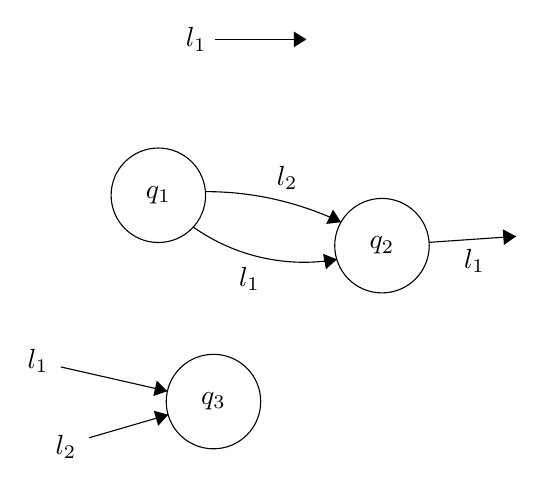
\begin{tikzpicture}[scale=0.2]
		\tikzstyle{every node}+=[inner sep=0pt]
		\draw [black] (19.7,-17.1) circle (3);
		\draw (19.7,-17.1) node {$q_1$};
		\draw [black] (33.9,-20.3) circle (3);
		\draw (33.9,-20.3) node {$q_2$};
		\draw [black] (23.2,-30.2) circle (3);
		\draw (23.2,-30.2) node {$q_3$};
		\draw [black] (31.038,-21.173) arc (-80.10211:-125.29706:12.173);
		\fill [black] (31.04,-21.17) -- (30.16,-20.82) -- (30.34,-21.8);
		\draw (25.49,-21.65) node [below] {$l_1$};
		\draw [black] (22.688,-16.869) arc (90.10901:64.49182:19.909);
		\fill [black] (31.3,-18.81) -- (30.79,-18.01) -- (30.36,-18.92);
		\draw (27.88,-16.76) node [above] {$l_2$};
		\draw [black] (36.89,-20.09) -- (42.41,-19.71);
		\fill [black] (42.41,-19.71) -- (41.57,-19.26) -- (41.64,-20.26);
		\draw (39.77,-20.48) node [below] {$l_1$};
		\draw [black] (13.5,-28) -- (20.27,-29.54);
		\draw (12.75,-27.61) node [left] {$l_1$};
		\fill [black] (20.27,-29.54) -- (19.6,-28.87) -- (19.38,-29.85);
		\draw [black] (15.3,-32.5) -- (20.32,-31.04);
		\draw (14.53,-33.08) node [left] {$l_2$};
		\fill [black] (20.32,-31.04) -- (19.41,-30.78) -- (19.69,-31.74);
		\draw [black] (23.3,-7.2) -- (29.1,-7.2);
		\draw (22.8,-7.2) node [left] {$l_1$};
		\fill [black] (29.1,-7.2) -- (28.3,-6.7) -- (28.3,-7.7);
	\end{tikzpicture}
\end{center}

The partial graphs have a lot in common with Glushkov's construction. Let $D\times W$ be the set of labels. Then $\Lambda$ function returns a single label $\Lambda(\psi) = (y,w)$, which looks very much like an instance of the epsilon edge $(\emptyset,y,w,\emptyset)$. The $B$ function is responsible for collecting initial atomic symbols $\omega\in\Omega$ and their labels $(y,w)\in D \times W$, which resembles partial edges with no source $(\emptyset,y,w,\omega)$. Similarly for $(\omega,y,w) \in E(\psi) \subset \Omega \rightharpoonup D \times W$, which we could interpret as partial edge with no target $(\omega,y,w,\emptyset)$. The set of 2-factors $L(\psi)\subset (\Omega \times \Omega \rightharpoonup D \times W)$ could be interpreted as a set of full labelled edges $\Omega \times D \times W \times \Omega$. As a result, instead of converting $\Lambda,B,E$ and $L$ to a subsequential transducer, we can directly obtain definition of a partial graph with no ``post processing'' required. This could be better seen if we combine all of the 
$\Lambda,B,E$ and $L$ functions into one large procedure $G$ that returns the entire partial graph $G : RE_W^{\Omega\rightarrow D} \rightarrow (\Omega,\delta)$. We have several cases to consider.

Let's recall how each function behaves on the atomic symbol $\omega$.
We can see that $G$ should return a partial graph with no full edges\\
$L(\epsilon) =  \emptyset$ \\
one outgoing edge \\
$E(\omega) =  \{(\omega,(\epsilon,0)) \}$  \\
one incoming edge \\
$B(\omega) =  \{(\omega,(\epsilon,0)) \}$ \\
and no epsilon edge \\
$\Lambda(\omega) = \emptyset$ \\
Hence it could be presented as the following very simple single-state graph:
\begin{center}
	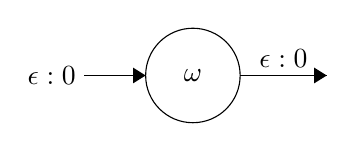
\begin{tikzpicture}[scale=0.2]
		\tikzstyle{every node}+=[inner sep=0pt]
		\draw [black] (26.6,-19) circle (3);
		\draw (26.6,-19) node {$\omega$};
		\draw [black] (19.7,-19) -- (23.6,-19);
		\draw (19.2,-19) node [left] {$\epsilon:0$};
		\fill [black] (23.6,-19) -- (22.8,-18.5) -- (22.8,-19.5);
		\draw [black] (29.6,-19) -- (35.1,-19);
		\fill [black] (35.1,-19) -- (34.3,-18.5) -- (34.3,-19.5);
		\draw (32.35,-18.5) node [above] {$\epsilon:0$};
	\end{tikzpicture}
\end{center}
In order to use such a graph as an automaton it's enough to treat all the outgoing edges state's subsequential output and the input label of every full or incoming edge is directly determined by the target state. Hence this graph becomes the following automaton:
\begin{center}
	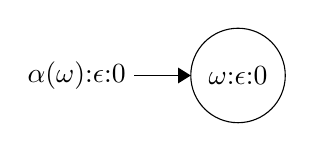
\begin{tikzpicture}[scale=0.2]
		\tikzstyle{every node}+=[inner sep=0pt]
		\draw [black] (26.6,-19) circle (3);
		\draw (26.6,-19) node {$\omega{:}\epsilon{:}0$};
		\draw [black] (20,-19) -- (23.6,-19);
		\draw (19.5,-19) node [left] {$\alpha(\omega){:}\epsilon{:}0$};
		\fill [black] (23.6,-19) -- (22.8,-18.5) -- (22.8,-19.5);
	\end{tikzpicture}
\end{center}
It is worth pointing out that there will always be at most only one outgoing edge per state and at most one global epsilon edge. This directly follows from the definition of $E$ as function $E(\psi): \Omega \rightharpoonup D \times W$ rather than relation $E(\psi): \Omega \times D \times W$ and because $\Lambda$ returns only a single element. 

The set $\Omega$ is directly treated as the set of states $Q$. An input string $\sigma_1\sigma_2...\sigma_n\in\Sigma^*$ is accepted by the partial graph if there exists a path $(\emptyset,y_0,w_0,\omega_1)\rightarrow(\omega_1,y_1,w_1,\omega_2)\rightarrow...\rightarrow(\omega_n,y_n,w_n,\emptyset)$ starting in incoming edge $(\emptyset,y_0,w_0,\omega_1)$, ending in outgoing edge $(\omega_n,y_n,w_n,\emptyset)$ and such that for every $i$ the input symbol $\sigma_i$ equals to the symbol of target state $\alpha(\omega_i)$.  The produced output is determined by $y_0y_1...y_n$.

It's possible to omit the use of $\alpha$ mapping entirely during the implementation. There is no need to linearise $\psi$ or build $\Omega$.
Instead we could use a special data structure of singly-linked graphs. Every vertex itself is an array holding its own outgoing (full) edges. Such representation of graphs has certain benefits. Unlike in most other graph data structures (adjacency matrices and lists) the singly-linked graphs don't have a well defined set of vertices. There could be millions of vertices allocated in computer memory and none of them connected to any other.  

\begin{center}
	\begin{tikzpicture}[scale=0.2]
		\tikzstyle{every node}+=[inner sep=0pt]
		\draw [black] (18.9,-20.9) circle (3);
		\draw (18.9,-20.9) node {$q_1$};
		\draw [black] (40.4,-15.9) circle (3);
		\draw (40.4,-15.9) node {$q_2$};
		\draw [black] (33.7,-37.3) circle (3);
		\draw (33.7,-37.3) node {$q_3$};
		\draw [black] (32.1,-26) circle (3);
		\draw (32.1,-26) node {$q_4$};
		\draw [black] (52.6,-21.1) circle (3);
		\draw (52.6,-21.1) node {$q_{54}$};
		\draw [black] (19,-32.3) circle (3);
		\draw (19,-32.3) node {$q_{11}$};
		\draw [black] (23.8,-12.4) circle (3);
		\draw (23.8,-12.4) node {$q_{99}$};
	\end{tikzpicture}
\end{center}
Each of those individual vertices could be thought of as a separate graph in and of itself but the distinction is blurry. As soon as we add some connection

\begin{center}
	\begin{tikzpicture}[scale=0.2]
		\tikzstyle{every node}+=[inner sep=0pt]
		\draw [black] (18.9,-20.9) circle (3);
		\draw (18.9,-20.9) node {$q_1$};
		\draw [black] (40.4,-15.9) circle (3);
		\draw (40.4,-15.9) node {$q_2$};
		\draw [black] (33.7,-37.3) circle (3);
		\draw (33.7,-37.3) node {$q_3$};
		\draw [black] (32.1,-26) circle (3);
		\draw (32.1,-26) node {$q_4$};
		\draw [black] (52.6,-21.1) circle (3);
		\draw (52.6,-21.1) node {$q_{54}$};
		\draw [black] (19,-32.3) circle (3);
		\draw (19,-32.3) node {$q_{11}$};
		\draw [black] (23.8,-12.4) circle (3);
		\draw (23.8,-12.4) node {$q_{99}$};
		\draw [black] (25.36,-14.96) -- (30.54,-23.44);
		\fill [black] (30.54,-23.44) -- (30.55,-22.5) -- (29.69,-23.02);
		\draw (27.31,-20.48) node [left] {$l_1$};
	\end{tikzpicture}
\end{center}
the two graphs suddenly merge into one (or perhaps, one is a subgraph of the other, since it's possible to reach $q_4$ from $q_99$ but not the other way around). We might think of one ``infinite supergraph''  containing all vertices that have ever been created or could potentially be created in the future. Hence it makes more sense to speak of connected components rather than the ``supergraph'' itself. Given some set of incoming partial transitions $B\subset \{\emptyset\} \times \mathbb{L} \times Q$, the connected component induced by $B$ is the set $\overline{B}$ defined as subset of $Q$ containing all the reachable vertices, starting from some initial edge in $B$.  

Every time we encounter some symbol $\sigma$, we allocate a new vertex $q$ and initialize it as an empty array $q=[]$. Next we create a set of incoming edges $B$ containing only a single edge $B=\{(\emptyset,\epsilon,0,q_1)\}$. Similarly we also need to keep track of outgoing edges $E=\{(q_1,\epsilon,0,\emptyset)\}$. The $G(\sigma)$ function will return a partial graph $(\overline{B},B \cup E)$ but for technical details (presented in upcoming paragraphs) the sets $B$ and $E$ should be kept in their own separate lists. There is  no need to store the full edges in their own list, since they are stored in each corresponding vertex. The set of vertices $\overline{B}$ is implied by $B$ and also doesn't need to be stored in computer memory explicitly. Hence $(\overline{B},B \cup E)$  is merely the formal presentation of a graph but in the actual implementation a data structure like $(B,E)$ is used instead. 

We have a full formal and algorithmic description of $G(\sigma)$. The next case to consider is the union $G(\psi_0 + \psi_1)$. We need to
combine the full edges from both subgraphs \\
$L(\psi_0 + \psi_1) = L(\psi_0)\cup L(\psi_1) $ \\
as well as the respective outgoing \\
$E(\psi_0 + \psi_1) = E(\psi_0)\cup E(\psi_1) $ \\
and incoming edges \\
$B(\psi_0 + \psi_1) = B(\psi_0)\cup B(\psi_1) $ \\
The epsilon edges cannot be combined in any way hence union might result in errors when both subgraphs simultaneously contain their own epsilon edges \\
$\Lambda(\psi_0+\psi_1) = \Lambda(\psi_0) \cup \Lambda(\psi_1)$ \\
We can combine all of those operations into a single operation $G$ on partial graphs. We first perform $G(\psi_0)$ and then $G(\psi_1)$. The result of $G(\psi_0 + \psi_1)$ does not require to perform any additional operations. The graph $G(\psi_0 + \psi_1)$ is merely one ``supergraph'' consisting of two disconnected components $G(\psi_0)$ and $G(\psi_1)$. Algorithmic implementation can be achieved by concatenating the list of incoming edges of the first subgraph with the other (and analogically for outgoing edges). Because we use singly-linked graphs as the backing data structure, the set of reachable vertices is automatically implied and does not require to be updated.
As a result union operation is $O(1)$ with respect to size of the graph and its memory footprint is kept low. 


The next case to consider is the concatenation $G(\psi_0 \psi_1)$. 
First we need to compute $G(\psi_0)$ to obtain the sets $B_{\psi_0}$, $E_{\psi_0}$, $L_{\psi_0}$ and $\Lambda_{\psi_0}$ of its incoming, outgoing, full and epsilon edges respectively. 
Analogically for $G(\psi_1)$. The $L$ function performs product \\
$\Lambda(\psi_0\psi_1) =\Lambda(\psi_0) \cdot \Lambda(\psi_1)$ \\
This operation can be redefined in terms of partial edges. If the set of labels $\mathbb{L}$ is a monoid, then multiplication of edges becomes possible.  Outgoing edge $(q_1,l_1,\emptyset)$ multiplied together with incoming edge $(\emptyset,l_2,q_2)$ will give us a full edge $(q_1,l_1 l_2 ,q_2)$. Similarly, multiplication of epsilon edge $(\emptyset,l_3,\emptyset)$ with either outgoing edge $(q_1,l_1,\emptyset)$ or incoming edge $(\emptyset,l_2,q_2)$ yields $(q_1,l_3 l_1,\emptyset)$ or $(\emptyset,l_3 l_2,q_2)$ respectively. If we extend those operations to work on entire sets of edges \\
$X \cdot Y = \{ x\cdot y : x\in X \mbox{ and }y\in Y\}$ \\
then we can introduce multiplication (concatenation) of partial graphs. \\
$G(\psi_0)\cdot G(\psi_1) = (\overline{B_{\psi_0}},L_{\psi_0}\cup L_{\psi_1} \cup E_{\psi_0} \cdot B_{\psi_1} \cup \Lambda_{\psi_0} \cdot B_{\psi_1} \cup E_{\psi_0} \cdot \Lambda_{\psi_1} \cup   \Lambda_{\psi_0} \cdot \Lambda_{\psi_1})$
In the context of singly-linked graphs, the operation $E_{\psi_0} \cdot B_{\psi_1}$ for every $(q_0,y_0,w_0,\emptyset)\in E_{\psi_0}$ and $(\emptyset,y_1,w_1,q_1)\in B_{\psi_1}$ computes a full edge $(q_0,y_0 y_1,w_0 w_1,q_2)$ and inserts it to the list $q_0$. Analogically partial edges are computed and inserted to the respective lists as well.

The case of Kleene closure $G(\psi_0 ^*)$ is similar to concatenation. When working with singly linked graphs, Kleen closure behaves like concatenation of graph $G(\psi_0) \cdot G(\psi_0)$ with itself, except that epsilon edges require special handling. 

The remaining cases of $G(\psi:d)$, $G(\psi w)$ and $G(w \psi)$ are achieved by multiplying outgoing edges with $(d,0)$, $(\epsilon,w)$ with incoming edges and outgoing edges with $(\epsilon,w)$ respectively. It should be noted that labels $\mathbb{L}$ can act on partial graphs. Left action $l \cdot G$ multiplies $l\cdot b$ with all incoming edges of $G$ and the epsilon edge $l \cdot \lambda$. Similarly right action $G \cdot l$  multiplies $e \cdot l$ with all outgoing edges of $G$ and the epsilon edge $ \lambda \cdot l$. 

We conclude this construction with a few notes about performance and possible extensions. As it can be noticed, by eliminating the need for computing linearised alphabet $\Omega$, the algorithm became fully parallelizable. Any subexpression of the original regular expression can be compiled independently to the rest. Singly-linked graphs guarantee that no reallocations of states are necessary. The weights and outputs only act on partial edges, hence once a full edge is computed it is never mutated. As a result, the algorithm never has the need to revisit already compiled parts of the automaton. In such sense the construction is fully linear and all individual operations are of $O(1)$ complexity. There are exactly as many states as there are input symbols, hence memory consumption is also linear. The produced automata are epsilon-free, except for the only one global partial epsilon edge. The compiled singly-linked graph forms an automaton in and of itself, hence no conversion from 2-factors to automata is necessary, like it was in the case of ``standard'' Glushkov's construction. Moreover, it's straightforward to extend the compilation with custom ``external'' functions \\
$G(F(\psi)) = F_{custom\_implementation}(G(\psi))$ \\
This allows for adding non-standard operations like subtraction, composition, inversion, powerset and many others.













\section{Code specification}

The exact implementation of most functions in Solomonoff requires deep technical understanding of automata theory. The examples and intuitive explanations provided at the beginning of this chapter convey the essence of most implementations. This section is meant to guide the reader through general code structure, conventions and their justification. 

The process of writing compilers is very different from a standard engineering process. The code must follow rigorous specification and there is little room for bugs. The development of Solomonoff, since the earliest stages could be shortly summarised as ``mathematically rigorous programming'', rather than ``ad-hoc software engineering''. Therefore our Java implementation follows strict conventions of contract-oriented programming. All preconditions, postconditions and invariants are asserted using runtime analysis. We also make extensive use of the  ``typeclass pattern''. Almost everything is an interface. Each of the interfaces corresponds to some formal mathematical definition and stores a handful of axioms (each axiom is a method). Non-axiom methods are canonically represented as pure static functions. 
For example consider a set of finite sequences $\Omega_X$ of elements from a set $X$. A string $\sigma_1\sigma_2\sigma_1$ over alphabet $\Sigma=\{\sigma_1,\sigma_2\}$ might be represented as a sequence $\langle \sigma_1,\sigma_2,\sigma_1\rangle$ of $\Omega_\Sigma$. An axiomatization of finite sequences might be a (dependent) pair $(n, f)$ of some number $n$ and function $f$ that to every integer between $0$ and $n$ assigns some element of $X$. Formally written as $(n, f) : \mathbb{N} \times (0...n \rightarrow X)$. Then in Java we could represent it as class
\begin{lstlisting}[language=java, escapeinside={(*}{*)}]
	class (*$\Omega$*)<X>{
		int n();
		X f(int i); //requires 0<=i<n
	}
\end{lstlisting}
Then a function that operates on $\Omega_X$, like concatenation for instance, would have to be represented using a pure static method.
\begin{lstlisting}[language=java, escapeinside={(*}{*)}]
	static <X> (*$\Omega$*)<X> concat((*$\Omega$*)<X> left, (*$\Omega$*)<X> right){...}
\end{lstlisting}
Sometimes, different implementations of $\Omega_X$ might use different underlying data structures, which in turn allow for more efficient implementations of certain functions. For example the generic implementation of \texttt{concat} might create a new instance with a new backing array and copy the elements of the two previous sequences. However, if we know that the exact implementation uses linked lists, a much more efficient procedure could work in constant time.  For this reason Solomonoff sometimes defines the non-axiomatic methods directly as part of interface, not because they are necessary, but because they can be implemented more efficiently. The programmer should still be aware of the underlying formal specification. 

Our Java code also strictly follows the specification of linear types. Even though Java compiler does not have any support for borrowing, ownership and lifetimes, that does not mean the code cannot be properly annotated in such a manner. For example consider the above definition of \texttt{concat}. It might produce a new instance for each call, but a more efficient implementation would mutate one of the arguments. The only problem is that mutations might lead to bugs and data races when not used properly. To avoid that, we explicitly specify (in the comments), which function arguments are linear.
For instance, if we specified that \texttt{left} argument is ``consumed'', then we should never use it after calling \texttt{concat}. Suppose that $\Omega_X$ is implemented using linked lists and the right argument is appended to the left one. We could write something like this to concatenate \texttt{a + b1 + b2}
\begin{lstlisting}[language=java, escapeinside={(*}{*)}]
	concat(a,b1);
	concat(a,b2);
\end{lstlisting}
but this solution might break as soon as the implementation is changed. The canonical way of writing code with linear types would be instead
\begin{lstlisting}[language=java, escapeinside={(*}{*)}]
	a2 = concat(a,b1);
	//a is consumed and should never be touched again!
	a3 = concat(a2,b2);
	//a2 is consumed and should never be touched again!
\end{lstlisting}
The programmer must also keep in mind that in order to invoke \texttt{concat(left,right)} we must also make sure that we own the \texttt{left} argument. If a reference to this variable was simultaneously used in some other place and we consumed it here, that other place would have no way of knowing that \texttt{left} is no longer valid. Therefore attention must be paid, whenever we copy references from one place to the other (which is commonly known as ``borrowing''). 

Every function that mutates its arguments, can also be represented as a linear function without mutations. For instance 
\begin{lstlisting}[language=java, escapeinside={(*}{*)}]
	static <X> void concat((*$\Omega$*)<X> left, (*$\Omega$*)<X> right)
\end{lstlisting}
is the mutating version of 
\begin{lstlisting}[language=java, escapeinside={(*}{*)}]
	/**consumes left*/
	static <X> (*$\Omega$*)<X> concat((*$\Omega$*)<X> left, (*$\Omega$*)<X> right)
\end{lstlisting}
In object-oriented languages we have one more possible approach
\begin{lstlisting}[language=java, escapeinside={(*}{*)}]
	void concat((*$\Omega$*)<X> right)
\end{lstlisting}
where \texttt{this} instance is implied to be linear (\texttt{this=left}).

In Solomonoff, the convention is to use the second approach for static functions, but the third approach whenever the method is part of an interface, although there are some exceptions. In particular, note that the static functions require all generic arguments to be mentioned explicitly. When there are too many of them, it becomes more convenient and readable to turn static methods into interface methods and let all the generics be declared only once globally as the interface generics. Instead of
\begin{lstlisting}[language=java, escapeinside={(*}{*)}]
	static <X1,X2,X3,Y> Y f1(X1 x1, X2 x2, X3 x3){...}
	static <X1,X2,X3,Y> Y f2(X1 x1, X2 x2, X3 x3){...}
\end{lstlisting}
we obtain more concise notation
\begin{lstlisting}[language=java, escapeinside={(*}{*)}]
	interface ShareGenerics<X1,X2,X3,Y>{
		default Y f1(X1 x1, X2 x2, X3 x3){...}
		default Y f2(X1 x1, X2 x2, X3 x3){...}
	}
\end{lstlisting}
This approach should be considered merely as syntactic sugar. Those functions are usually not meant to be extended in any way. Most of the methods in Solomonoff are pure and do not have any state. Even the seemingly impure functions become pure when linear logic is taken into account. 







